%********************************************************************
\chapter{Reflood Simulation using TRACE Code}\label{ch:trace_reflood}
%********************************************************************

% Opening paragraph
Reflood phase is the last phase of the 4 canonical phases in the mitigation of \glsfirst[hyper=false]{lbloca} in a \gls[hyper=false]{lwr}.
It refers to the phase of the transient in which emergency coolant water flows slowly upward through the dried reactor core, quenching the fuel elements along the way, preventing them from having further damage due to overheating.

% This Chapter and its Overview
This chapter introduces the phenomenology of reflood and its modeling in the thermal-hydraulics system code \gls[hyper=false]{trace}.
Section~\ref{sec:reflood_trace} first presents a quick overview of the \gls[hyper=false]{trace} code,
including a major simplification the code takes to describe a complex two-phase flow in the reactor coolant circuit during accident scenarios.
Section~\ref{sec:reflood_phenomenology} then describes the reflood in \glspl[hyper=false]{lwr}: its importance, its phenomenology, and its modeling.
It introduces several important terminologies used throughout the thesis.
The description is focused from the perspective of the \gls[hyper=false]{trace} code and is by no means an exhaustive account on the subject. 

The present study is based on the data from a \glsfirst[hyper=false]{setf} for reflood experiment.
The \glsfirst[hyper=false]{feba} facility and the relevant test runs for this study are described Section~\ref{sec:reflood_feba_setf}.
The modeling aspects of the facility in the \gls[hyper=false]{trace} is then detailed in Section~\ref{sec:reflood_feba_trace}.

Section~\ref{sec:reflood_initial_inputs_selection} deals with the problem of selecting the initial set of input parameters perceived to be influential for the simulation.
Afterward, prior uncertainties in the form of \glspl[hyper=false]{pdf} are assigned to the selected input parameters.
Those two steps provide the starting point for the application of sensitivity and uncertainty analyses on the \gls[hyper=false]{trace} model of \gls[hyper=false]{feba} presented in the upcoming chapters.
Section~\ref{sec:reflood_prior_uq} presents the propagation of the specified prior uncertainties on the \gls[hyper=false]{trace} model to assess the initial level of uncertainty in the predictions before any experimental data is used to update the prior uncertainties.
Lastly, Section~\ref{sec:reflood_chapter_summary} concludes and summarizes the chapter. 

\section{Thermal-Hydraulics System Code \glsentryshort{trace}}\label{sec:reflood_trace}

\gls[hyper=false]{trace} is the best-estimate system \gls[hyper=false]{th} code developed by the \gls[hyper=false]{usnrc} 
as a tool for light water reactor transient analysis during normal and accident scenarios.
Its development is an on-going effort 
to modernize into a single software package all previous \gls[hyper=false]{usnrc} \gls[hyper=false]{th} codes
that were developed separately for specific reactor types and/or applications.
This ultimately would make the code more versatile for end users and more efficient to maintain for the developer.

\subsection{Thermal-hydraulics System Code}\label{sub:th_system_code}

% What is system code
Thermal-hydraulics system code is a computer code used to analyze the thermal-hydraulics behavior of \glspl[hyper=false]{npp} \cite{Roth2014}.
\marginpar{thermal-hydraulics system code}
Its current usage ranges from safety analysis and licensing process of current reactor designs to qualification of a new reactor design \cite{Petruzzi2008, Petruzzi2016}.
To that end, the code is designed to be a comprehensive tool capable of simulating wide range of operating conditions, 
from normal operations, anticipated transients, to accident scenarios foreseen in nuclear power plant operation.

% Component-based system code
Nuclear reactor system is a complex system of numerous interconnected components, each serving distinct purpose, built with multiple engineered safety features.
During a transient, the system might exhibit complex behavior with important physical phenomena interacting at vastly different time scales ($10^{-1} \, [s]$ in a power excursion due to control rod ejection, $10^5 \, [s]$ for decay heat removal after successful reactor shutdown) and
length scales ($10^{-3} \, [mm]$ for boiling at sub-channel level, $10^3 \, [m]$ for coolant flow in the primary/secondary circuit).
Additionally, the engineered safety features are designed for some equipments (such as control rods, valves, pump, etc.) to perform safety-related action.
Such equipments, in turn, is controlled by a complex dynamical control system.
As such, system code has to take into account these different aspects to properly simulate the thermal-hydraulics behavior of nuclear power plants.
Indeed, com\-ponent-based codes, such as \gls[hyper=false]{trace}, approach the problem by representing each prominent component in nuclear reactor system separately.
On top of a two-phase fluid dynamics equation solver, system code includes models for steam separator, pump, heat exchanger, valve, pressurizer, and neutron-kinetics 
as well as comprehensive models for control system to mimic the signal monitoring and component action actuation systems in a \gls[hyper=false]{npp}.   
System thermal-hydraulics thus distinguishes itself by considering explicitly the geometry, materials, boundary conditions, various interconnecting components, and control systems that constitute an \gls[hyper=false]{npp} \cite{DAuria2012}.
\begin{figure}[bth]
	\centering
	\includegraphics[scale=0.50]{../figures/nuclearTHSystem/nuclearTHSystem.pdf}
	\caption[Illustration of Heated Channel]{}
	\label{fig:nuclear_th_system}
\end{figure}

% The essence of the problem tackled in thermal-hydraulics system code
However, it can be argued that the modeling of two-phase flow inside a heated channel remains a central part in nuclear thermal-hydraulics analysis 
\marginpar{basic thermal-hydraulics, two-phase flow in a heated channel}
which puts an emphasis in the correct prediction of cladding temperature evolution during different postulated scenarios. 
This is also supported by the fact that the majority of operating nuclear power plants is of \gls[hyper=false]{lwr} type, 
where two-phase flow can be expected to occur during its operation, both in normal operating and accident condition for \glspl[hyper=false]{bwr} and in accident condition for \glspl[hyper=false]{pwr}.
\begin{figure}[bth]
	\centering
	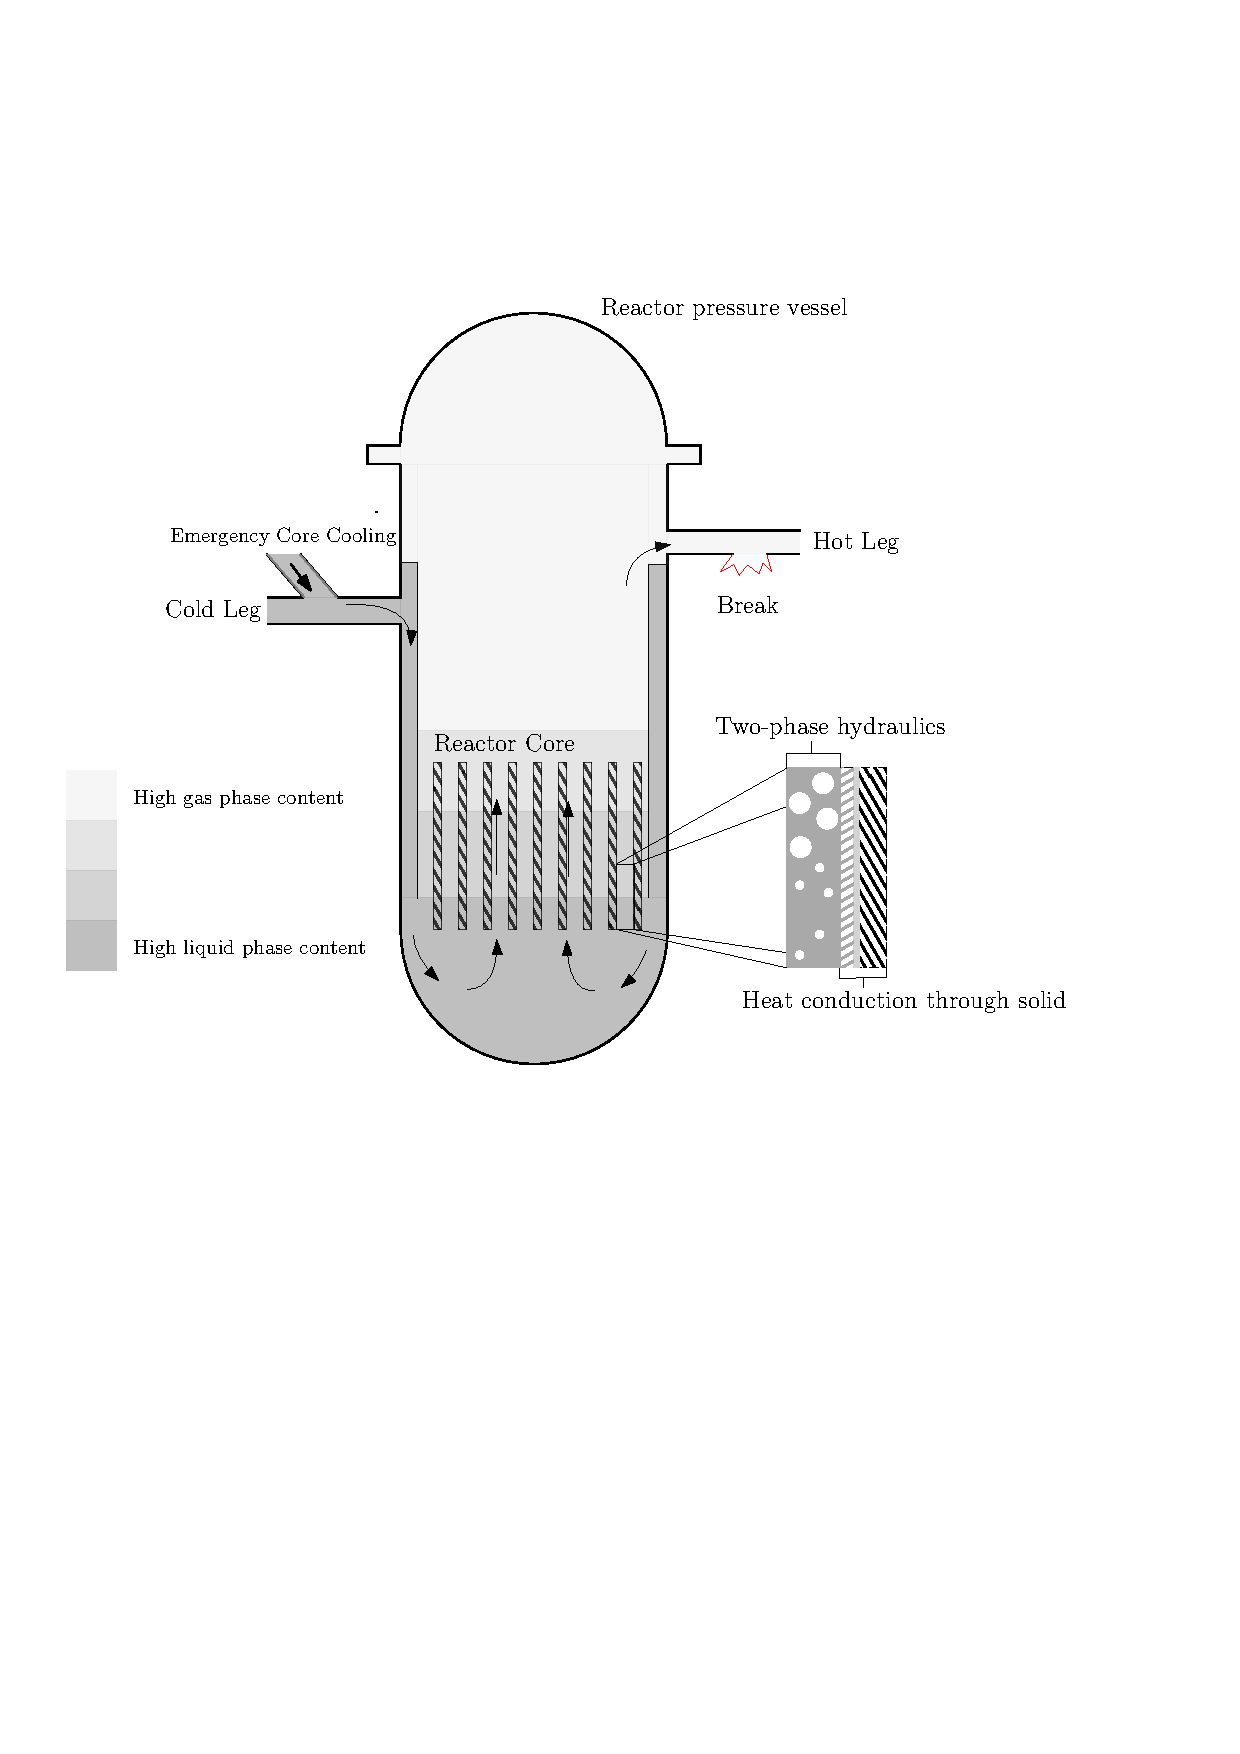
\includegraphics[scale=0.55]{../figures/heatedChannel/heatedChannel.pdf}
	\caption[Illustration of Heated Channel]{System thermal-hydraulics analysis encompasses many aspects of nuclear reactor system analysis, but the core of the problem for predicting the cladding temperature evolution (especially during accident condition) is to model properly and realistically the coolant flow in a heated channel in steady or transient condition. Here it is shown a simplified picture of loss of coolant accident in a \glsentryshort{pwr} where phase change along the heated channel occurs.}
	\label{fig:heated_channel}
\end{figure}

% Major difficulty
This remaining problem of modeling properly the two-phase flow in a heated channel, though much more limited in scope, is by no means trivial.
\marginpar{flow regimes}
This due to the fact that in two-phase flow, the morphological configurations of the flow (i.e., \emph{flow regimes}) can vary widely depending on many parameters such as difference in phase density, phasic velocity, and flow orientation.
Different morphological configuration implies different interfacial surface structure between the two phases (see Fig.~\ref{fig:flow_regimes}), 
which in turn affects the mass, momentum, and energy coupling terms (\emph{transfer relation}) between the phases.
At the same time, the interfacial surface and its deformation in an arbitrary flow configuration are not known \emph{a priori} and becomes part of the solution.
\begin{figure}[bth!]
	\centering
	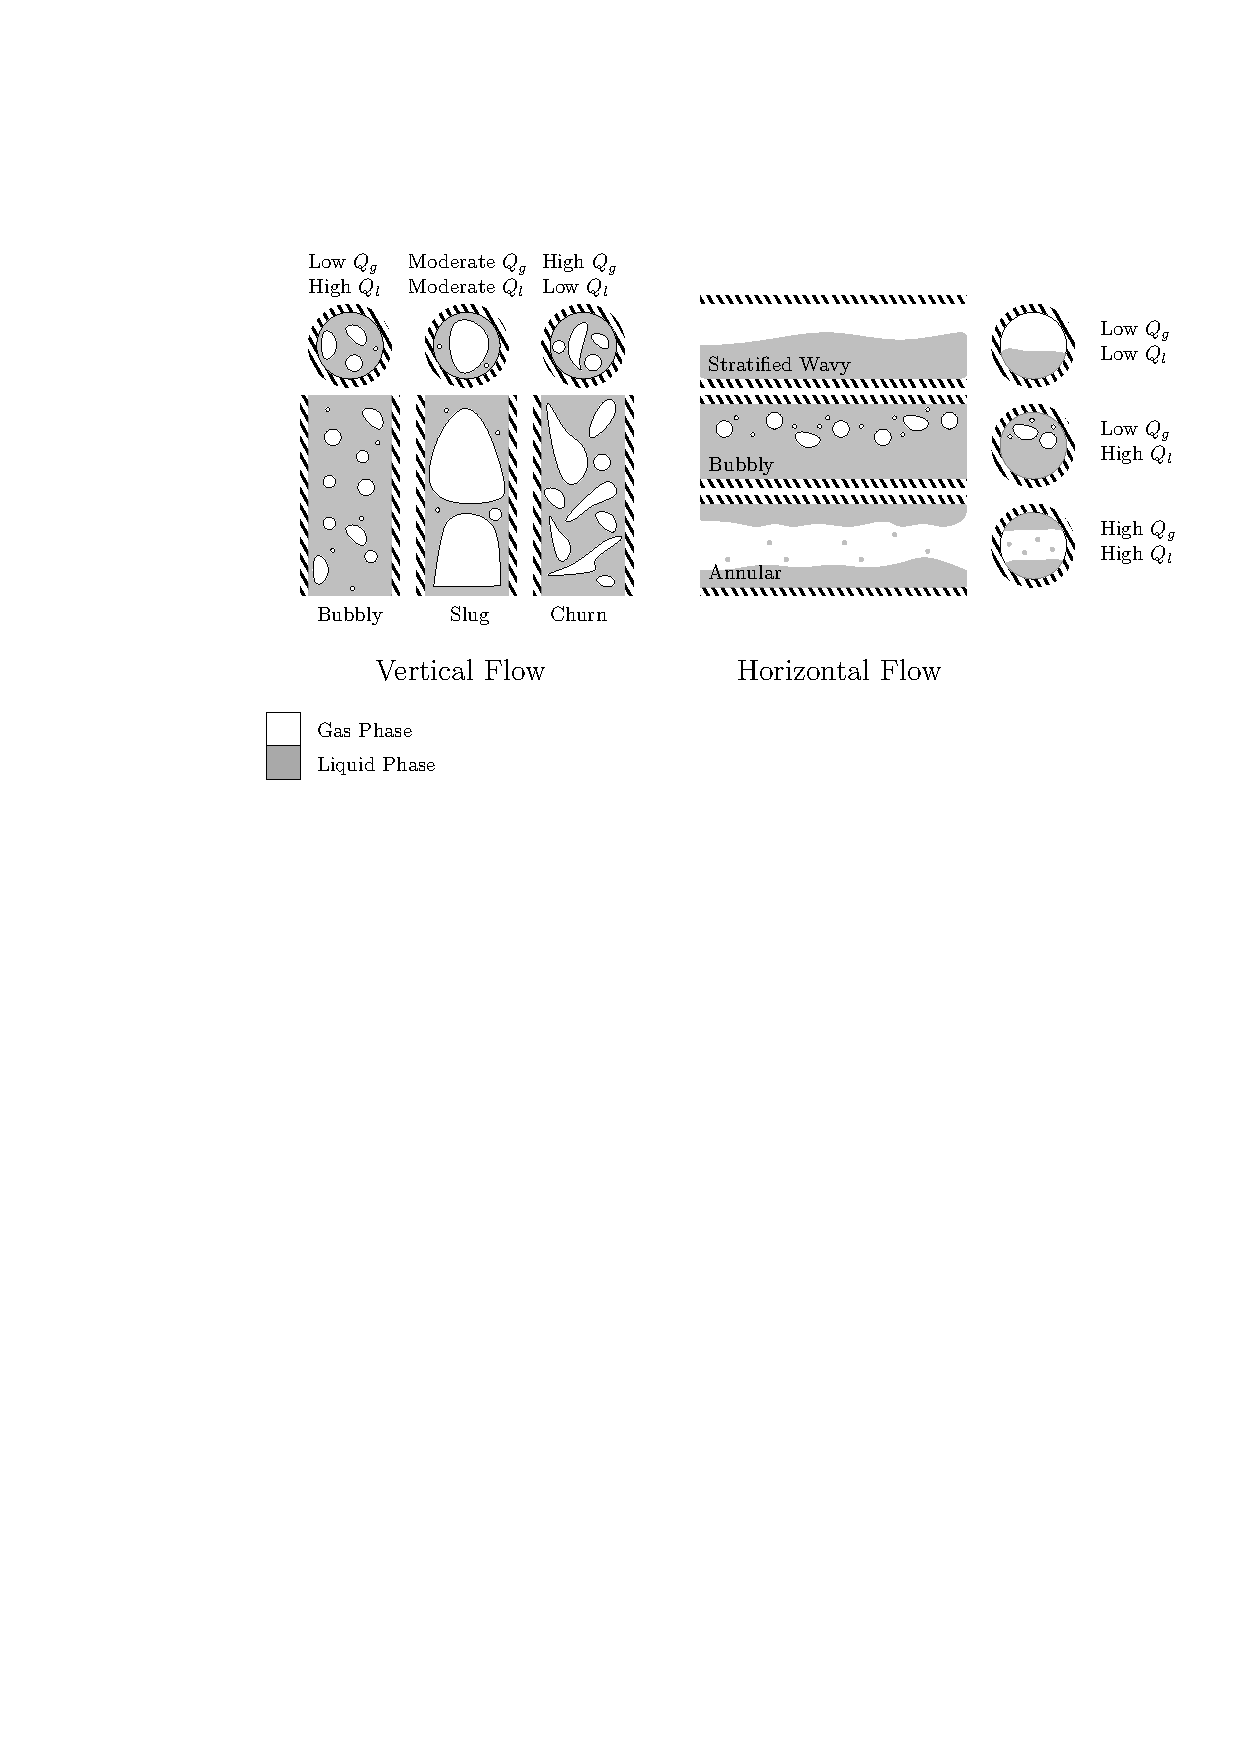
\includegraphics[width=\textwidth]{../figures/flowRegimes/flowRegimes.pdf}
	\caption[Some of the observed flow regimes in vertical and horizontal flow]{Some of the observed flow regimes in vertical and horizontal flow with different superficial liquid velocity, $Q_l = V_l / A$, and superficial gas velocity, $Q_g = V_g / A$, where $A$ is the flow area. The flows of both phases are co-current.}
	\label{fig:flow_regimes}
\end{figure}

% The rigorous approach, local instantaneous formulation
The most rigorous approach in describing two-phase flow is by using local instantaneous formulation where a set partial differential equations describing the conservation of mass, momentum, and energy, is formulated for each phase.
The two phases are, in turn, separated by zero-thickness interfacial surface.
The resulting set of equations fully describe the flow at any given location at any given time.
In addition to that, the solution of this formulation also respect the \emph{topological constraint} of the flow.
\marginpar{local instantaneous formulation, topological constraint}
The constraint states that only one phase can exist at any given time and at any given location in the flow \cite{Ghiaasiaan2007}.
This is illustrated in the Fig.~\ref{fig:phase_indicator_probe} where a hypothetical probe is put within a two-phase flow and a signal of indicator function $M(\mathbf{r}, t)$ is recorded.
\begin{figure}[bth!]
	\centering
	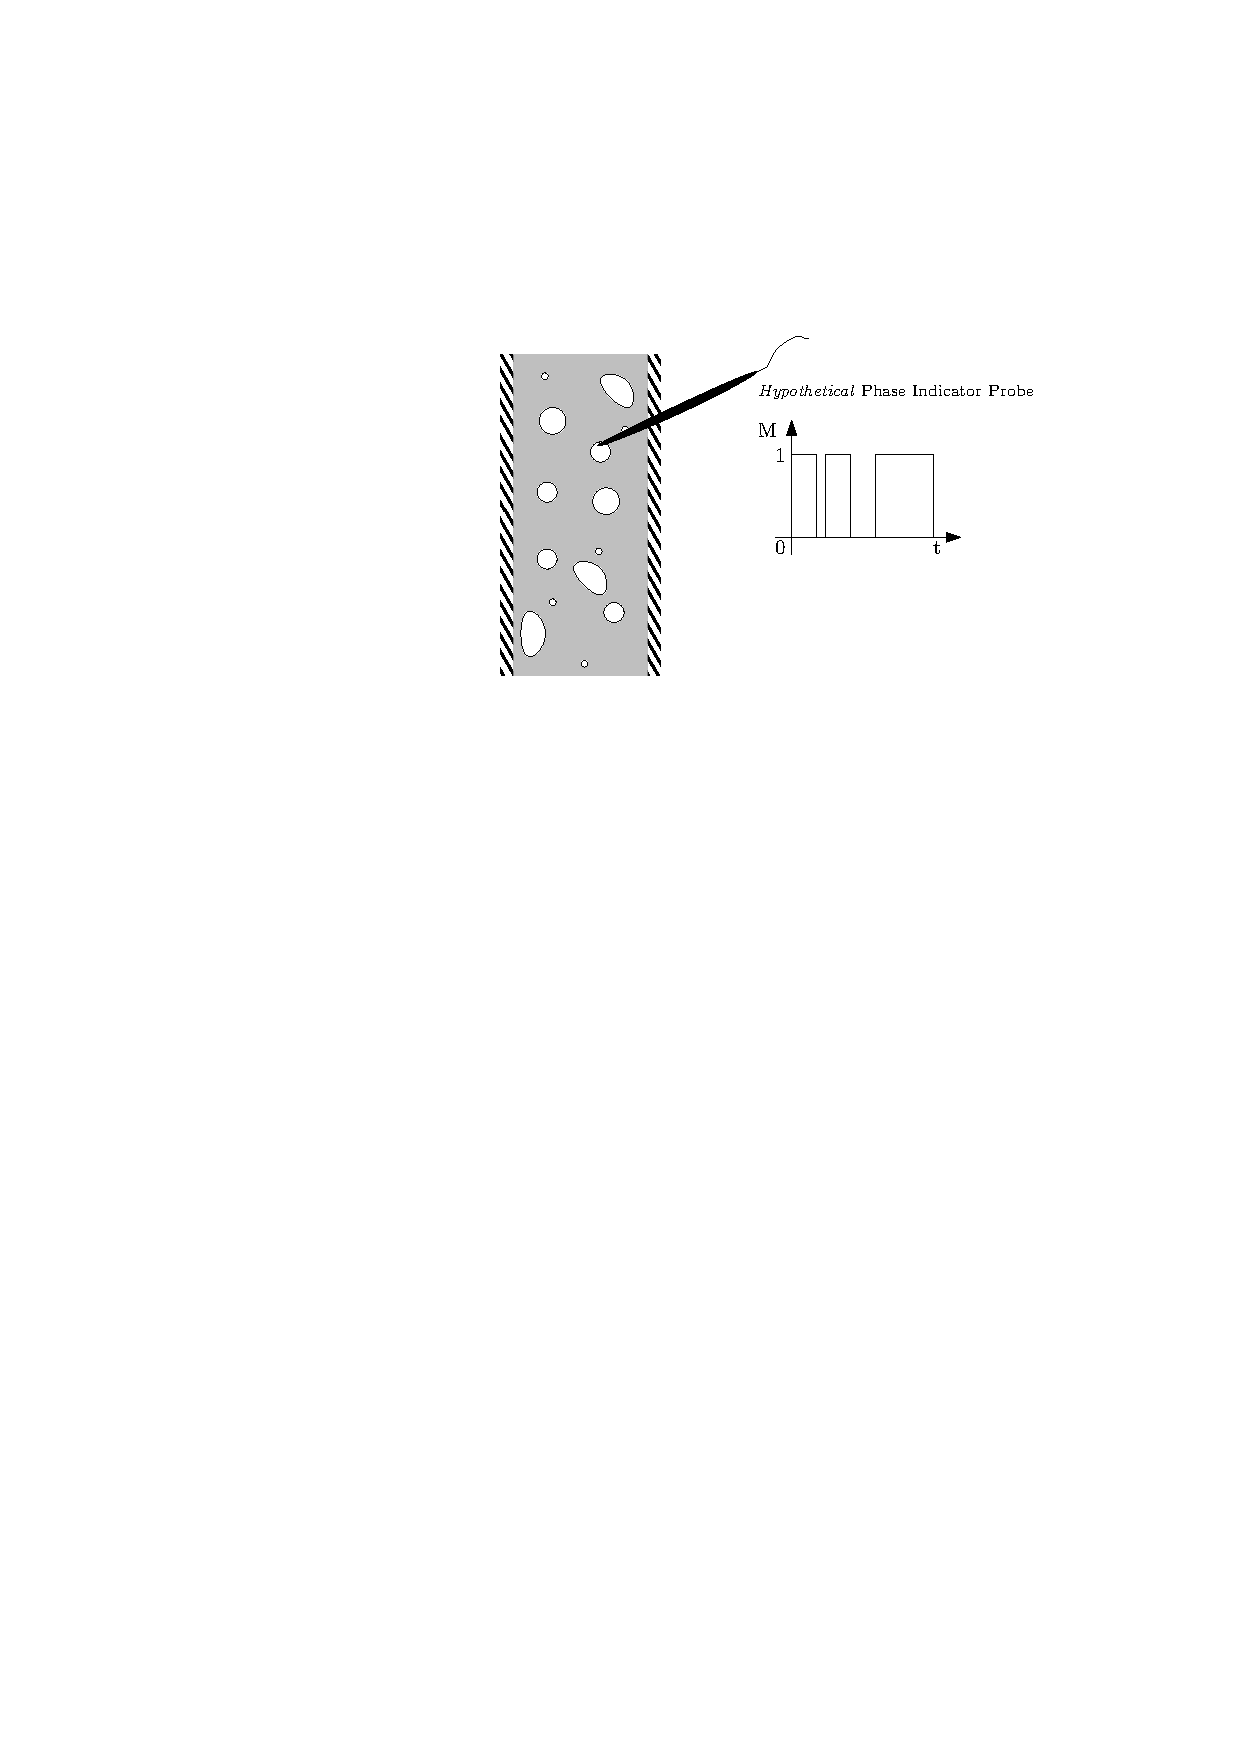
\includegraphics[scale=0.70]{../figures/phaseIndicatorProbe/phaseIndicatorProbe.pdf}
	\caption[A hypothetical phase indicator probe inside a channel of a two-phase flow]{Illustration of a hypothetical phase indicator probe inside a channel of a two-phase flow, recording at a point location the indicator function value (Eq.~(\ref{eq:indicator_function})) at every instance.}
	\label{fig:phase_indicator_probe}
\end{figure}
The indicator function is defined as,
\begin{equation}
  M (\mathbf{r}, t) =
    \begin{cases}
      1 \, ; \, \text{if probe tip in \text{gas phase}} \\
      0 \, ; \, \text{otherwise}
    \end{cases}
\label{eq:indicator_function}
\end{equation}
where \gls[hyper=false]{r} is vector of position;
and \gls[hyper=false]{t} is time.
The indicator function defined here is equivalent to the local instantaneous void fraction, 
which can be interpreted as the probability that the gas phase is present at a given point in space at a given moment \cite{USNRC2012}. 

As mentioned, the interfacial surface structure of the flow determines the coupling terms between the two phases.
\marginpar{resolving the motion of interfacial surface}
However, this surface and its deformation along the flow are not known \emph{a priori}.
As such, the solution of local instantaneous formulation of two-phase flow requires the motion of interfacial surface to be simultaneously resolved. 
As the time and length scales of the interfacial structure in a two-phase flow of an arbitrary morphological configurations can vary wildly,
the problem of resolving the motion of interfacial surface becomes intractable. 
Though advances have been made in the area of Computational Fluid Dynamics (CFD) in this regard, 
the problem remains intractable for the purpose of thermal-hydraulics system analysis (see \cite{Bestion2014} for recent review on the topic).

% The simplified approach, Time and Volume Averaged
To simplify the intractability problem of resolving the motion of interfacial surface motion in two-phase flow, 
time- and volume-average is carried out on the flow.
\marginpar{Time- and Volume-averaging}
Averaging can be seen as a filtering operation to remove the local temporal and spatial fluctuations (short scale variation) in the flow.
The length and duration which define short scale variation are problem specific 
(that is, at least qualitatively, not longer than the length and time scales of the flow configuration of interest).
The volume over which averaging is carried out is referred to either as a \emph{control volume}, a \emph{cell}, or a \emph{node}.

Averaging the indicator function both in time and in volume gives the void fraction,
\begin{equation}
  \langle \bar{\alpha} \rangle =  \frac{1}{\Delta V \Delta t} \int_{V}^{V + \Delta V} \int_{t}^{t + \Delta t} \alpha(\mathbf{r}, t) d\mathbf{r} dt = \frac{1}{\Delta V} \int_{V}^{V + \Delta V} \overline{\alpha(\mathbf{r})} d\mathbf{r}
\label{eq:void_fraction}
\end{equation}
Following the above formulation, void fraction can be interpreted as the fraction of the control volume occupied by the gas phase \cite{USNRC2012}. 
In the subsequent section the angle brackets and the overbar will be dropped from the void fraction notation 
and any mention of void fraction will refer to the time- and volume-averaged formulation given above.

% Two fluid model and its closure
Averaging the flow state variables in time and volume and using them to formulate a set of mass, momentum, and energy balance equations describing the fluid dynamics yield the so-called \emph{two-fluid model} \cite{Ishii2011}.
\marginpar{Time- and Volume-Averaged formulation, two-fluid model}
The model is the state of the art formulation for describing the dynamics of two-phase flow in system codes (which include, for example CATHARE, RELAP5, and \gls[hyper=false]{trace}).
This model separately treats the transport phenomena of the two phases of fluid resulting in six balance equations 
which are able to capture phenomena where thermal and mechanical non-equilibrium conditions exist between the two phases, conditions to be expected in wide range of \gls[hyper=false]{npp} transients.
\begin{figure}[bth]
	\centering
	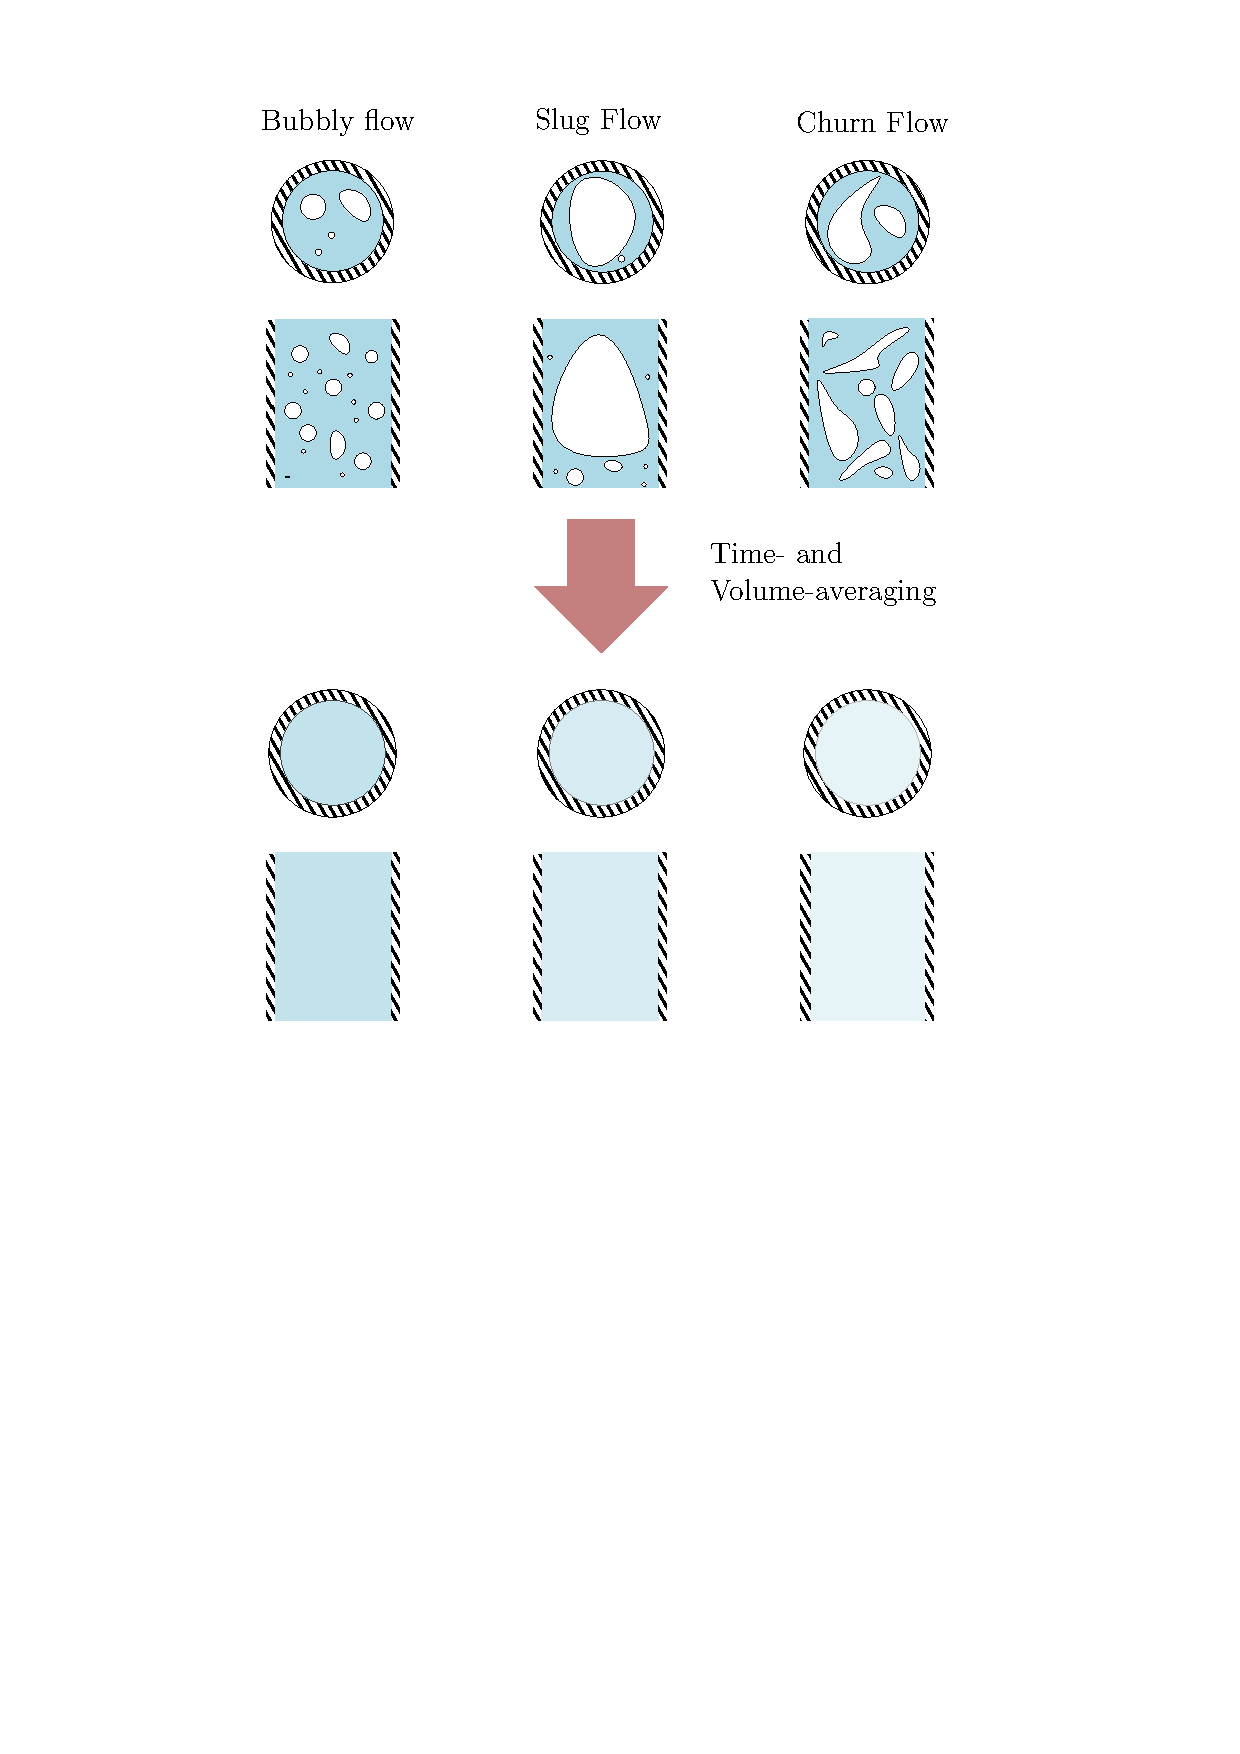
\includegraphics[scale=0.55]{../figures/flowAveraging/flowAveraging.pdf}
	\caption[Illustration of Flow Averaging]{Time and volume average carried out on the two-phase flow inside a channel results in a tractable form of fluid dynamics equation, but incur loss of information at the local level, especially when it comes to the interfacial structure between the two phases.}
	\label{fig:flow_averaging}
\end{figure}

% Closing paragraph
The next section will summarize the final formulation of the governing equations (time- and volume-averaged) adopted in \gls[hyper=false]{trace}, of which the complete derivation can be found in \cite{USNRC2012}.
As the averaging incurs loss of information regarding the flow local information (such as the interfacial structure between the phases, see Fig.~\ref{fig:flow_averaging}), 
the transfer relations between the two phases have to be recovered through the use of closure models briefly described in Section~\ref{sub:closure_and_flow_regimes}.

\subsection{Governing Equations}\label{sub:governing_equations}

As mentioned, the hydraulic module of \gls[hyper=false]{trace} is based on a two-fluid six-equation model, 
solving the conservation equations of mass, momentum, and energy for the liquid and vapor phases in the coolant \cite{USNRC2012}.
Furthermore, the formulations are given in volumetric term (i.e., per unit volume basis) with a reference to a select control volume (or \emph{node}).
A symbol is defined the first time it appears in an equation 
and the complete list of symbols can be found in the \hyperref[app:notations]{Glossary of Notations} at back of the thesis.

\paragraph{Mass balance equations, liquid and gas phases:}
\begin{equation}
	\frac{\partial [(1-\alpha)\rho_l]}{\partial t} + \nabla \cdot [(1-\alpha) \rho_l \mathbf{v_l}] = - \Gamma
\label{eq:mass_balance_liquid}
\end{equation}
\begin{equation}
	\frac{\partial [\alpha \rho_g]}{\partial t} + \nabla \cdot [\alpha \rho_g \mathbf{v_g}] = \Gamma
\label{eq:mass_balance_gas}
\end{equation}
where the subscripts indicate the phase, $l$ for the liquid phase and $g$ for the gas phase (vapor); 
\gls[hyper=false]{alpha} is the void fraction; 
\gls[hyper=false]{rhol} (\gls[hyper=false]{rhog}) is the mass density of the liquid (gas) phase;
and \gls[hyper=false]{vl} (\gls[hyper=false]{vg}) is the flow velocity of the liquid (gas) phase.
The terms in either sides of the two mass balance equations are explained in Table~\ref{tab:mass_balance}.

\begin{table}[ht]
	\myfloatalign
	\caption[The terms in \glsentryshort{trace} two-fluid model mass balance equations]{The terms in \glsentryshort{trace} two-fluid model mass balance equations (all are given in volumetric term)}
	\label{tab:mass_balance}
	\begin{tabularx}{\textwidth}{Xcc} 
		\toprule
		\tableheadline{Terms} & \tableheadline{Liquid Phase} & \tableheadline{Gas Phase} \\ 
		\midrule
		\footnotesize{mass rate of change}  					 & $\frac{\partial [(1-\alpha)\rho_l]}{\partial t}$  & $\frac{\partial [\alpha \rho_g]}{\partial t}$ \\
		\footnotesize{mass convection rate} 					 & $\nabla \cdot [(1-\alpha) \rho_l \mathbf{v_l}]$   & $\nabla \cdot [\alpha \rho_g \mathbf{v_g}]$ \\
		\midrule
		\footnotesize{interfacial mass-transfer rate}  & $- \Gamma$                                        & $\Gamma$ \\
		\bottomrule
	\end{tabularx}
\end{table}

Note that the term \gls[hyper=false]{Gamma}, the volumetric interfacial mass-transfer rate,
is given with a convention that it is positive for the transfer from liquid phase to gas phase.
This term is defined in Eq.~(\ref{eq:Gamma}) below.

\paragraph{Momentum balance equations, liquid and gas phases:}
\begin{equation}
	\begin{split}
		& \frac{\partial [(1-\alpha)\rho_l \mathbf{v}_l]}{\partial t} + \nabla \cdot [(1-\alpha) \rho_l \mathbf{v_l} \otimes \mathbf{v_l}] + (1 - \alpha) \nabla p \\
		& \quad = \mathbf{f}_i + \mathbf{f}_{wl} + (1 - \alpha) \rho_l \mathbf{g} - \Gamma \mathbf{v}_i
	\end{split}
\label{eq:momentum_balance_liquid}
\end{equation}
\begin{equation}
	\begin{split}
		& \frac{\partial [\alpha \rho_g \mathbf{v}_g]}{\partial t} + \nabla \cdot [\alpha \rho_g \mathbf{v_g} \otimes \mathbf{v_g}] + \alpha \nabla p \\
		& \quad = - \mathbf{f}_i + \mathbf{f}_{wg} + \alpha \rho_g \mathbf{g} + \Gamma \mathbf{v}_i
	\end{split}
\label{eq:momentum_balance_gas}
\end{equation}
where $\nabla p$ is the pressure gradient;
\gls[hyper=false]{fi} is the volumetric force due to shear at the phase interface;
\gls[hyper=false]{fwl} is the volumetric force acting on the liquid phase due to shear at the wall (i.e., fluid-structure contact);
\gls[hyper=false]{fwg} is the volumetric force acting on the gas phase due to shear at the wall;
\gls[hyper=false]{gravity} is the gravitational acceleration;
and \gls[hyper=false]{vinterface} is the flow velocity at the phase interface.
Table~\ref{tab:momentum_balance} lists the terms in either sides of the two momentum balance equations.

\begin{table}[ht]
	\myfloatalign
	\caption[The terms in \glsentryshort{trace} two-fluid model momentum balance equations]{The terms in \glsentryshort{trace} two-fluid model momentum balance equations (all are given in volumetric term)}
	\label{tab:momentum_balance}
	\begin{tabularx}{\textwidth}{>{\raggedright}Xcc} 
		\toprule
		\tableheadline{Terms} & \tableheadline{Liquid Phase} & \tableheadline{Gas Phase} \\ 
		\midrule
		\footnotesize{momentum rate of change}  					 	& $\frac{\partial [(1-\alpha)\rho_l \mathbf{v}_l]}{\partial t}$  				& $\frac{\partial [\alpha \rho_g \mathbf{v}_g]}{\partial t}$ \\
		\footnotesize{momentum convection rate} 					 	& $\nabla \cdot [(1-\alpha) \rho_l \mathbf{v_l} \otimes \mathbf{v_l}]$ 	& $\nabla \cdot [\alpha \rho_g \mathbf{v_g} \otimes \mathbf{v_g}]$ \\
		\footnotesize{pressure gradient}                  	& $(1 - \alpha) \nabla p$                                        				& $\alpha \nabla p$ \\
		\midrule
		\footnotesize{momentum change due to:}            	&                                                                 			& \\
		\footnotesize{interfacial friction} 								& $\mathbf{f}_i$ 																												&  $- \mathbf{f}_i$ \\
		\footnotesize{wall friction} 						  					& $\mathbf{f}_{wl}$ 																										& $\mathbf{f}_{wg}$ \\
		\footnotesize{body force} 													& $(1 - \alpha) \rho_l \mathbf{g}$ 																			& $\alpha \rho_g \mathbf{g}$ \\
		\footnotesize{interfacial mass-transfer} 	  				& $- \Gamma \mathbf{v}_i$ 																							& $\Gamma \mathbf{v}_i$ \\
		\bottomrule
	\end{tabularx}
\end{table}

Note that the formulation in \gls[hyper=false]{trace} uses the simplifying assumption of $p_i = p_g = p_l$.
That is, the pressure in a given control volume is the same in either phases as well as at the interface \cite{USNRC2012}.

For the friction (shear) terms in right hand side, TRACE uses the following formulations,
\begin{equation}
	\mathbf{f}_i = C_i (\mathbf{v}_g - \mathbf{v}_l) |\mathbf{v}_g - \mathbf{v}_l| 
\label{eq:fi}
\end{equation}
\begin{equation}
	\mathbf{f}_{wl} = - C_{wl} \mathbf{v}_l |\mathbf{v}_l|
\label{eq:fwl}
\end{equation}
\begin{equation}
	\mathbf{f}_{wg} = - C_{wg} \mathbf{v}_g |\mathbf{v}_g|
\label{eq:fwg}
\end{equation}
where the friction coefficients \gls[hyper=false]{cint}, \gls[hyper=false]{cwl}, \gls[hyper=false]{cwg} for interfacial shear, wall-liquid shear, and wall-gas shear, 
respectively are obtained from flow regime-dependent empirical correlations.

\paragraph{Energy balance equations, liquid and gas phases:}
\begin{equation}
	\begin{split}
		& \frac{\partial [(1-\alpha)\rho_l(e_l + |\mathbf{v_l}|^2/2]}{\partial t} + \nabla \cdot \left[(1-\alpha) \rho_l \left(e_l+\frac{P}{\rho_l}+\frac{|\mathbf{v_l}|^2}{2}\right) \mathbf{v_l} \right] \\
		&	\quad = q_{il} + q_{wl} + q_{wsat} + q_{dl} + (1 - \alpha) \rho_l \mathbf{g} \cdot \mathbf{v}_l \\
		& \qquad - \Gamma h^\prime_l + (\mathbf{f}_{i} + \mathbf{f}_{wl}) \cdot \mathbf{v}_l
	\end{split}
\label{eq:energy_balance_liquid}
\end{equation}
\begin{equation}
	\begin{split}
		 & \frac{\partial [\alpha \rho_g (e_g + |\mathbf{v_g}|^2/2]}{\partial t} + \nabla \cdot \left[\alpha \rho_g \left(e_g+\frac{P}{\rho_g}+\frac{|\mathbf{v_g}|^2}{2}\right) \mathbf{v_g} \right] \\
		 & \quad  = q_{ig} + q_{wg} + q_{dg} + \alpha \rho_g \mathbf{g} \cdot \mathbf{v}_g + \Gamma h^\prime_g + (-\mathbf{f}_{i} + \mathbf{f}_{wg}) \cdot \mathbf{v}_g
	\end{split}
\label{eq:energy_balance_gas}
\end{equation}
where \gls[hyper=false]{el} (\gls[hyper=false]{eg}) is the liquid (gas) phase internal energy;
\gls[hyper=false]{qil} (\gls[hyper=false]{qig}) is the volumetric interfacial heat transfer on the liquid (gas) phase;
\gls[hyper=false]{qwl} (\gls[hyper=false]{qwg}) is the volumetric wall (sensible) heat transfer on the liquid (gas) phase;
\gls[hyper=false]{qwsat} is the volumetric wall (latent) heat transfer on the liquid phase;
\gls[hyper=false]{qdl} (\gls[hyper=false]{qdg}) is the volumetric direct power deposition on the liquid (gas) phase;
\gls[hyper=false]{hlp} is the bulk liquid enthalpy;
and \gls[hyper=false]{hgp} is the gas phase saturation enthalpy.
Table~\ref{tab:energy_balance} lists all of the terms in either sides of the two energy balance equations.

\begin{table}[ht]
	\myfloatalign
	\caption[The terms in \glsentryshort{trace} two-fluid model energy balance equations]{The terms in \glsentryshort{trace} two-fluid model momentum energy equations (all are given in volumetric term)}
	\label{tab:energy_balance}
	\begin{tabularx}{\textwidth}{>{\raggedright}Xcc} 
		\toprule
		\tableheadline{Terms} & \tableheadline{Liquid Phase} & \tableheadline{Gas Phase} \\ 
		\midrule
		\footnotesize{energy rate of change}  						& $\frac{\partial [(1-\alpha)\rho_l(e_l + |\mathbf{v_l}|^2/2]}{\partial t}$  																											& $\frac{\partial [\alpha \rho_g (e_g + |\mathbf{v_g}|^2/2]}{\partial t}$ \\
		\footnotesize{energy convection rate} 						& \tiny{$\nabla \cdot \left[(1-\alpha) \rho_l \left(e_l+\frac{P}{\rho_l}+\frac{|\mathbf{v_l}|^2}{2}\right) \mathbf{v_l} \right]$} & \tiny{$\nabla \cdot \left[\alpha \rho_g \left(e_g+\frac{P}{\rho_g}+\frac{|\mathbf{v_g}|^2}{2}\right) \mathbf{v_g} \right]$} \\
		\midrule
		\footnotesize{(sensible) interfacial heat transfer} 	& \footnotesize{$q_{il}$}																									& \footnotesize{$- \mathbf{f}_i$} \\
		\footnotesize{(sensible) wall heat transfer} 					& \footnotesize{$q_{wl}$}																									& \footnotesize{$\mathbf{f}_{wg}$} \\
		\footnotesize{(latent) wall heat transfer} 						& \footnotesize{$q_{w\text{sat}}$} 																				& \footnotesize{$\alpha \rho_g \mathbf{g}$} \\
		\footnotesize{direct heat deposition} 								& \footnotesize{$q_{dl}$}																									& \footnotesize{$\Gamma \mathbf{v}_i$} \\
		\footnotesize{energy loss (gain) due to:} 						&                                                                         & \\
		\footnotesize{gravity}      													& \footnotesize{$(1 - \alpha) \rho_l \mathbf{g} \cdot \mathbf{v}_l$} 			& \footnotesize{$\alpha \rho_l \mathbf{g} \cdot \mathbf{v}_l$} \\
		\footnotesize{phase change} 													& \footnotesize{$- \Gamma h^\prime_l$} 																		& \footnotesize{$\Gamma h^\prime_g$} \\
		\footnotesize{wall and interfacial friction} 					& \footnotesize{$(\mathbf{f}_{i} + \mathbf{f}_{wl}) \cdot \mathbf{v}_l$} 	& \footnotesize{$(-\mathbf{f}_{i} + \mathbf{f}_{wg}) \cdot \mathbf{v}_g$}\\
		\bottomrule
	\end{tabularx}
\end{table}

The heat transfer terms between the wall and the phases follow Newton's law of cooling,
\begin{equation}
	q_{wl} = h_{wl} \, a_{wl} \, (T_w - T_l)
\label{eq:qwl}
\end{equation}
\begin{equation}
	q_{wg} = h_{wg} \, a_{wg} \, (T_w - T_g)
\label{eq:qwg}
\end{equation}
\begin{equation}
	q_{w\text{sat}} = h_{w\text{sat}} \, a_{wl} \, (T_w - T_\text{sat})
\label{eq:qwsat}
\end{equation}
where \gls[hyper=false]{tw}, \gls[hyper=false]{tl}, \gls[hyper=false]{tg}, \gls[hyper=false]{tsat} are the wall, liquid phase, liquid phase, and liquid saturation temperatures, respectively;
\gls[hyper=false]{awl} (\gls[hyper=false]{awg}) is the volumetric surface contact area between the wall and liquid (gas) phase (or \emph{the interfacial area concentration});
and \gls[hyper=false]{hwl}, \gls[hyper=false]{hwg}, and \gls[hyper=false]{hwsat} are the \glspl[hyper=false]{htc} between wall and liquid, wall and gas, and wall-saturated liquid, respectively.
The volumetric surface contact area as well as the heat transfer coefficients are obtained from a set of flow regime-dependent empirical correlations.

Additionally, the heat transfer terms at the interface between the two phases are also modeled using the same law,
\begin{equation}
	q_{il} = h_{il} \, a_{i} \, (T_{sg} - T_l)
\label{eq:qil}
\end{equation}
\begin{equation}
	q_{ig} = \frac{p_g}{p} \, h_{ig} \, a_{i} \, (T_{sg} - T_g)
\label{eq:qig}
\end{equation}
where \gls[hyper=false]{hil} (\gls[hyper=false]{hig}) is the \gls[hyper=false]{htc} for liquid (gas) phase at the interface;
\gls[hyper=false]{ai} is the volumetric interfacial surface area;
\gls[hyper=false]{pg} is the partial pressure of the gas phase;
and \gls[hyper=false]{tsg} is the saturation temperature corresponding to partial pressure of the gas phase.

Finally, the mass-transfer rate at the interface is defined using a thermal-energy jump condition that results in
\begin{equation}
	\Gamma = \frac{-(q_{ig} + q_{il}) + q_{w\text{sat}}}{(h^\prime_g - h^\prime_l)}
\label{eq:Gamma}
\end{equation}
In other words, the net heat transfer rate given to the saturated liquid phase, is used entirely for phase change.

\paragraph{}

Besides the set balance equations that govern the two-phase fluid flow,
\gls[hyper=false]{trace} also includes a heat conduction module (known as \emph{heat structure} component) 
to model correctly the heat transfer process in solid structures (e.g., active fuel, internal passive structures, etc.) 
and between the surface of such structures and the contacting fluid.
\paragraph{Heat conduction equation, solid structures:}
\begin{equation}
	\rho_s \, C_{ps} \frac{\partial T}{\partial t} - \nabla \cdot (k_s \nabla T) = q_s 
\label{eq:conduction}
\end{equation}
where \gls[hyper=false]{rhos} is the solid structure mass density;
\gls[hyper=false]{cps} is the solid structure thermal capacity;
\gls[hyper=false]{ks} is the solid structure thermal conductivity;
and $q_s$ is the volumetric heat source term in the solid.

At the contact between fluid and solid material, the total heat flux is given as,
\begin{equation}
	q'' = h_{wl} \, (T_{w} - T_l) + h_{w\text{sat}} \, (T_w - T_\text{sat}) + h_{wg} \, (T_w - T_g)
\label{eq:conduction_surface}
\end{equation}
where the heat flux at the surface of the structure, $q''$ is partitioned to different phases of the fluid, either as sensible or latent heat.
As can be seen, 
Eq.~(\ref{eq:conduction_surface}) couples the heat conduction equation with energy balance equations of the fluid through the terms defined in Eqs.~(\ref{eq:qwl}), (\ref{eq:qwg}), and (\ref{eq:qwsat}).

\subsection{Closure and Flow Regimes}\label{sub:closure_and_flow_regimes}

In each of the balance equations given above, 
the right hand side represents the source and sink terms mainly due to fluid interaction with solid structure (\emph{wall})
and the interaction between the phases, among others.
The set of balance equations characterizes exactly the two-phase flow inside a control volume in a time- and volume-averaged manner provided that the terms in the right hand side of the equation (such as, Eqs.~(\ref{eq:fi})-(\ref{eq:fwg}) and Eqs.~(\ref{eq:qwl})-(\ref{eq:qig})) are correct.

%**************************************************************************************
\section{Phenomenology and Modeling of Bottom Reflood}\label{sec:reflood_phenomenology}
%**************************************************************************************

% Opening Paragraph, the reflood phase
As mentioned in the opening of this chapter, reflood phase is the last phase of the four canonical phases in the mitigation of \gls[hyper=false]{lbloca} in \glspl[hyper=false]{lwr},
\marginpar{Reflood phase in LBLOCA}
in which emergency coolant water flows slowly upward through the reactor core, quenching the fuel elements along the way.
The phase is expected to occur after the refill phase, in which a successful injection of the water through the downcomer and lower plenum of the \gls[hyper=false]{rpv}.

% Reflooding
\emph{Quenching} (or \emph{rewetting}) refers to the phenomenon in which a sustainable contact between the liquid phase of the coolant and the hot surfaces of the fuel is re-established.
\marginpar{Quenching}
Prior to the quenching, the excessively high surface temperature prevents a stable contact between the liquid phase and the surface, degrading the heat transfer between the two.
The maximum temperature for which the liquid might make a stable contact with the surface is referred to as the \emph{quenching temperature}.
In consequence, although the bulk of the flow through the core is liquid, the inability for the liquid to make contact with the surface keeps it at a very high temperature \cite{Hewitt2000,Zeng2010}.

In \gls[hyper=false]{bwr}, reflood might also occurs by spraying the core from the top resulting in the \emph{top reflood};
\marginpar{Top and bottom reflood}
while in both \gls[hyper=false]{bwr} and \gls[hyper=false]{pwr}, injection of water downward through the downcomer and upward through the core is termed \emph{bottom reflood}.
There are different physical processes associated with the two, such as the fact that in the top reflood there is steam flow from the bottom of the channel pushing back the liquid injection.
This thesis is only concerned with the bottom reflood. 
As the process sets a limiting ability for the emergency coolant to bring about efficient cooling to the fuel elements in the \gls[hyper=false]{lbloca} transient, a proper modeling of the physical processes associated with the reflood phase is an important for the safety analysis of \glspl[hyper=false]{lwr}.

% Reflood curve
A typical mid-height cladding temperature evolution in a channel undergoing a bottom reflood 
\marginpar{Reflood curve}
(so-called \emph{reflood curve}) can be seen in Fig.~\ref{fig:ch2_reflood_curve_qois} under a constant coolant injection rate and a constant power boundary condition.
\begin{figure}[bth]
    \centering
    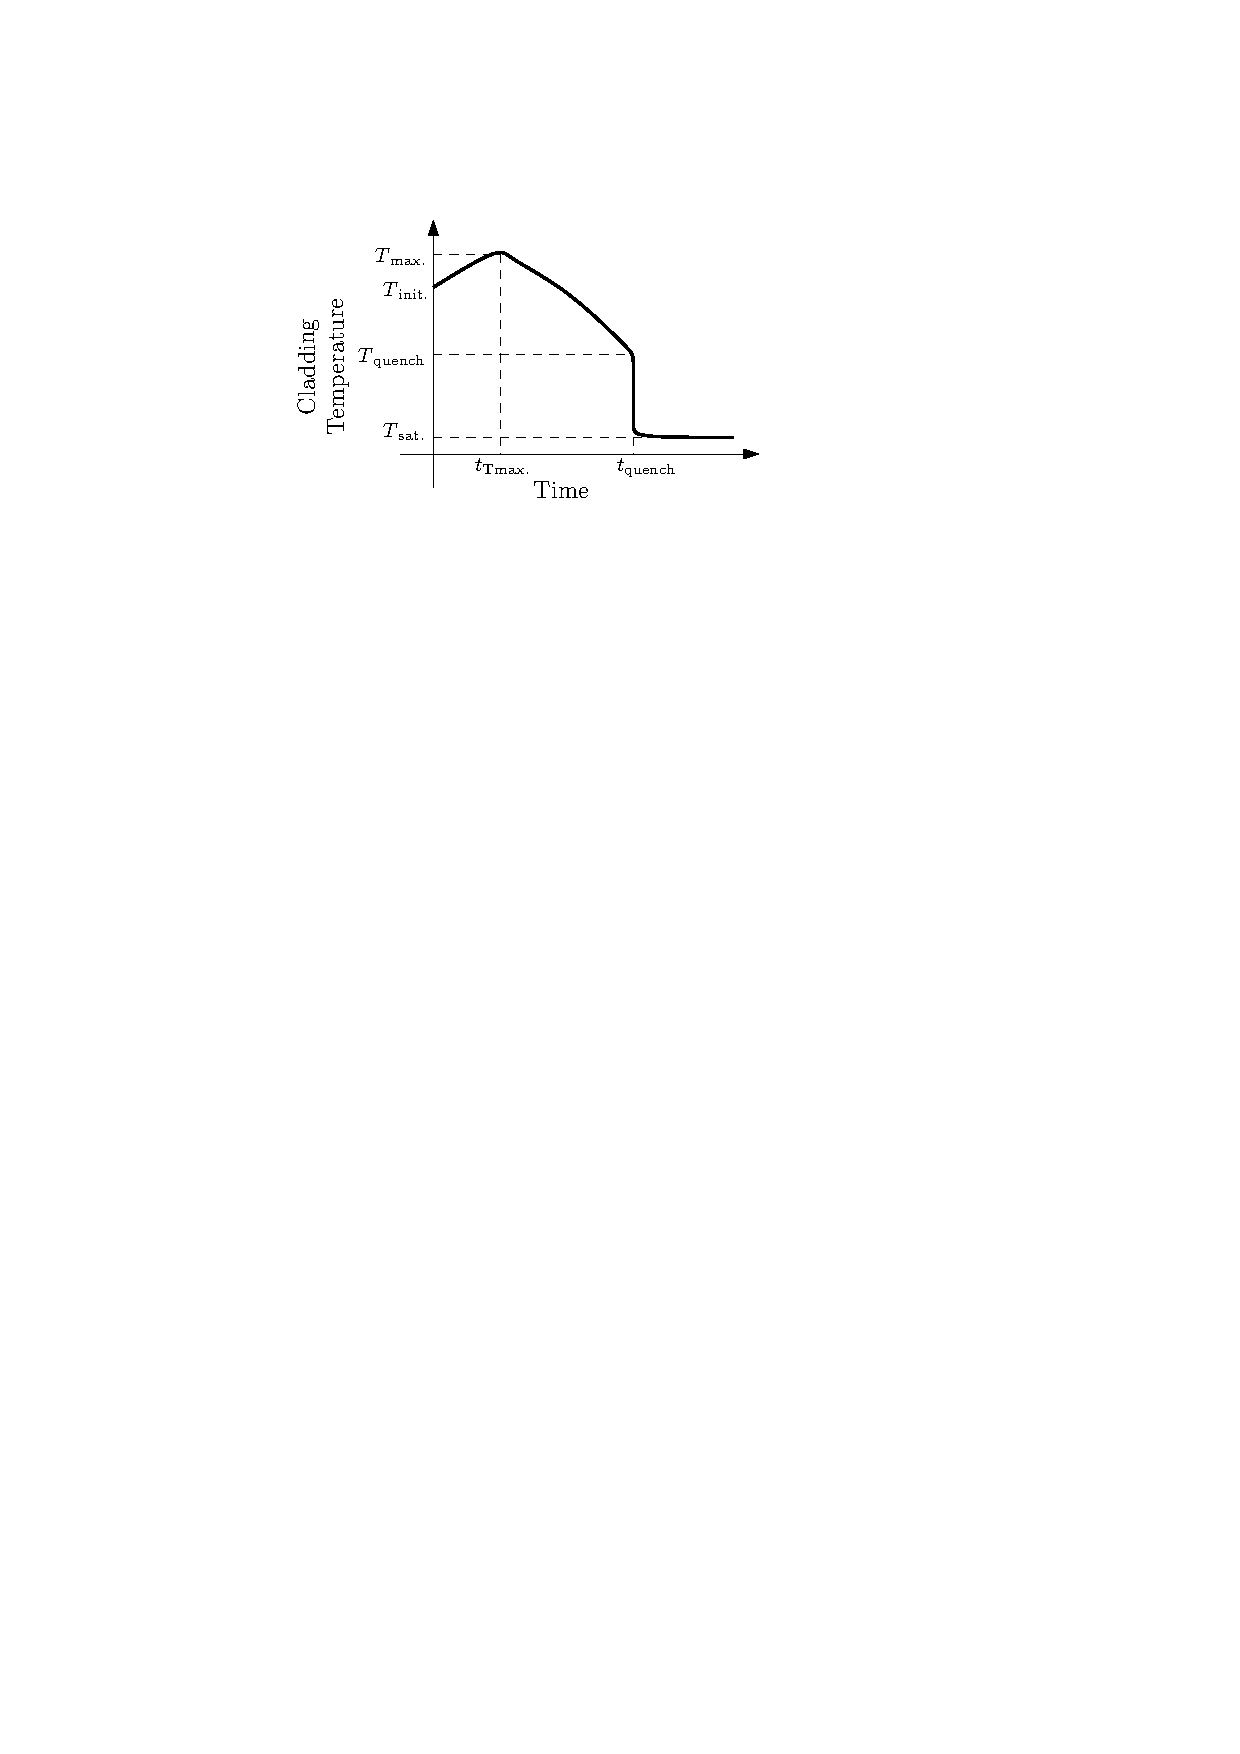
\includegraphics[width=1.0\textwidth]{../figures/chapter2/figures/refloodCurveQoIs}
    \caption[A typical cladding temperature evolution during constant flooding rate reflooding at mid-height assembly.]{A typical cladding temperature evolution during constant flooding rate reflooding at mid-height assembly (adapted from \cite{Zeng2010}). The labels on the both axes are typical \glspl[hyper=false]{qoi} of reflood transient, where the abbreviations $max.$, $init.$, and $sat.$ refer to the \emph{maximum}, \emph{initial}, and \emph{saturation}, respectively.}
    \label{fig:ch2_reflood_curve_qois}
\end{figure}

At the start of the transient (cladding temperature at $T_\text{init.}$) the channel consists purely of steam.
Keeping the power constant increases the cladding temperature up until mixture of steam and liquid (droplets) arrives at the location, improving the heat transfer mechanism, and decreasing the temperature ($T_\text{max.}$ at $t_{T_\text{max.}}$).
As the channel keeps undergoing reflood from the bottom, more droplets are available at the location to keep decreasing the cladding temperature.
Moreover, as the quenching happens below this particular location, large axial temperature gradient in the cladding is present and is further accelerating the heat conduction from the un-quenched part to the quenched part of the cladding.
Finally, when the temperature of the cladding reaches the quenching temperature ($T_\text{quench}$ at $t_{\text{quench}}$)), quenching occurs and stable contact between liquid and the cladding can be established.
From that point onward, the cladding temperature is in equilibrium with the liquid at saturation.

% The Modeling of The Phenomenology
The phenomenological view of the process, adopted by \gls[hyper=false]{trace} code \cite{USNRC2012}, is shown in Fig.~\ref{fig:ch2_post_chf_regime} along with the corresponding part in the reflood curve of Fig.~\ref{fig:ch2_reflood_curve}.
\marginpar{Reflood, phenomenology}
The post-\gls[hyper=false]{chf} flow regimes (regimes $(2)$--$(5)$ in the figure) are in-between two pre-\gls[hyper=false]{chf} flow regimes, namely nucleate boiling at the bottom and steam convection at the top.
\normdoublefigure[pos=!h,
                  mainlabel={fig:ch2_reflood_phenomenology},
                  maincaption={Phenomenology of flow during reflood according to \gls[hyper=false]{trace} code and the corresponding part of the transient in the reflood curve.},
				mainshortcaption={Phenomenology of flow during reflood according to \gls[hyper=false]{trace} code.},
                  leftopt={width=0.45\textwidth},
                  leftlabel={fig:ch2_post_chf_regime},
                  leftcaption={post-\gls[hyper=false]{chf} flow regimes $(2)$--$(5)$},
                  %leftshortcaption={},%
                  rightopt={width=0.5\textwidth},
                  rightlabel={fig:ch2_reflood_curve},
                  rightcaption={Reflood curve}]
{../figures/chapter2/figures/postCHFRegime}
{../figures/chapter2/figures/refloodCurvePhenomenology}

% Steam Flow
Consider a case of injecting subcooled liquid water with a constant feed rate (i.e., \emph{flooding rate}) into a dry heated channel.
At the given location of the temperature probe at the start of the transient, steam convection (regime~($2$) in Fig.~\ref{fig:ch2_post_chf_regime}) is the dominant heat transfer mechanism and the cladding temperature keeps increasing.
In \gls[hyper=false]{trace}, the steam convection process belongs to the pre-\gls[hyper=false]{chf} package \cite{USNRC2012}.

% DFFB
As the bottom part of the channel is quenched (the point of quenching on the surface is referred to as \emph{quench front}) three flow regimes can be observed.
\marginpar{\Glsfirst[hyper=false]{dffb}}
Far from the quench front, liquid droplets are dispersed and carried away by the bulk steam flow.
The flow regime, called \glsfirst[hyper=false]{dffb}, provides an improved heat transfer mechanism from the wall to the fluid as compared to the pure steam convection through direct radiation to the droplets, convection to the droplets and convection to the steam.
The droplets provide additional heat sink from the bulk steam flow.
The presence of the droplets in the flow also further enhance the turbulence of the steam flow improving the convection from the wall to the steam flow \cite{Zeng2010}.
The improvement to heat transfer brought by these mechanisms allows the cladding temperature to reach a maximum and decrease.

% Inverted Slug
As the quench front progresses upward, not too far from the front a more efficient cooling is provided from morphologically less regular entrained liquid, called ligaments or slugs (regime~($3$) in Fig.~\ref{fig:ch2_post_chf_regime}).
\marginpar{Inverted Slug}
Due to this efficient cooling, the cladding temperature keeps decreasing.
The slug flow regime is inverted in the sense that the slugs are of the liquid phase. 
In \gls[hyper=false]{trace} these slugs are modeled as prolate ellipsoids.
The flow regime itself represents an interpolatory region between the previous \glsentryshort{dffb} flow regime and the subsequent \gls[hyper=false]{iafb} flow regime \cite{USNRC2012}.

% IAFB
Closer to the front, the bulk of the subcooled liquid flow starts to appear in front of the surface.
\marginpar{\Glsfirst[hyper=false]{iafb}}
However, a thin vapor film still separates the liquid from the wall and thus prevents an ideal heat transfer to occur.
In this so-called \glsfirst[hyper=false]{iafb} flow regime (regime~($4$) in Fig.~\ref{fig:ch2_post_chf_regime}), the bulk of the coolant flow in the center of the channel is liquid (i.e., the liquid core).
The heat transfer mechanism from the wall is through convection to the vapor film and direct radiation to the liquid core \cite{Zeng2010,USNRC2012}.

% Transition Boiling
Finally, as quenching becomes imminent and the cladding temperature reaches the quenching temperature, the flow regime switch to the unstable \emph{transition boiling}, which literally means the transition between dry wall and wet wall regimes.
\marginpar{Transition boiling}
In \gls[hyper=false]{trace} the heat transfer is evaluated based on the look-up table \gls[hyper=false]{chf} at the particular flow conditions.
It results in a very large \gls[hyper=false]{htc} between the wall and the fluid and causes the rapid drop (i.e., quenching) of the temperature (regime~($5$) in Fig.~\ref{fig:ch2_post_chf_regime}). 
After quenching, the cladding surface is in full contact with the liquid.
The cladding temperature is in equilibrium with the bulk flow of saturated liquid and the flow regime involves different phenomena, namely nucleate boiling (regime~($6$) in Fig.~\ref{fig:ch2_post_chf_regime}).
In \gls[hyper=false]{trace}, as the steam convection, the nucleate boiling process belongs to the pre-\gls[hyper=false]{chf} package \cite{USNRC2012}.
%********************************************************************************
\section{FEBA Reflood Separate Effect Test Facility}\label{sec:reflood_feba_setf}
%********************************************************************************

% Introductory paragraph
A series of \gls[hyper=false]{feba} experiments was conducted in the 1980s at the Karlsruhe Institute of Technology (KIT)\footnote{formerly Kernforschungzentrum Karlsruhe (KfK)}
to improve the knowledge of the \gls[hyper=false]{ht} mechanism during reflooding,
taking into account the effects of spacer grids and flow blockage due to fuel rod ballooning.
The data from the facility was also intended to validate the \gls[hyper=false]{th} models and codes available at the time.

% FEBA Facility
The facility consisted of a test section with full height $5 \times 5$ bundle of \textsc{PWR} fuel rod simulator (Fig.~\ref{fig:feba_setf}a) enclosed in a rectangular stainless steel housing (Fig.~\ref{fig:feba_setf}b).
An approximate cosine power profile was mapped over of the height of the fuel rod simulators (Fig.~\ref{fig:feba_setf}c).
Seven spacer grids were used to provide mechanical support of the fuel rod simulators (Fig.~\ref{fig:feba_setf}d).

\begin{figure}[bth]
	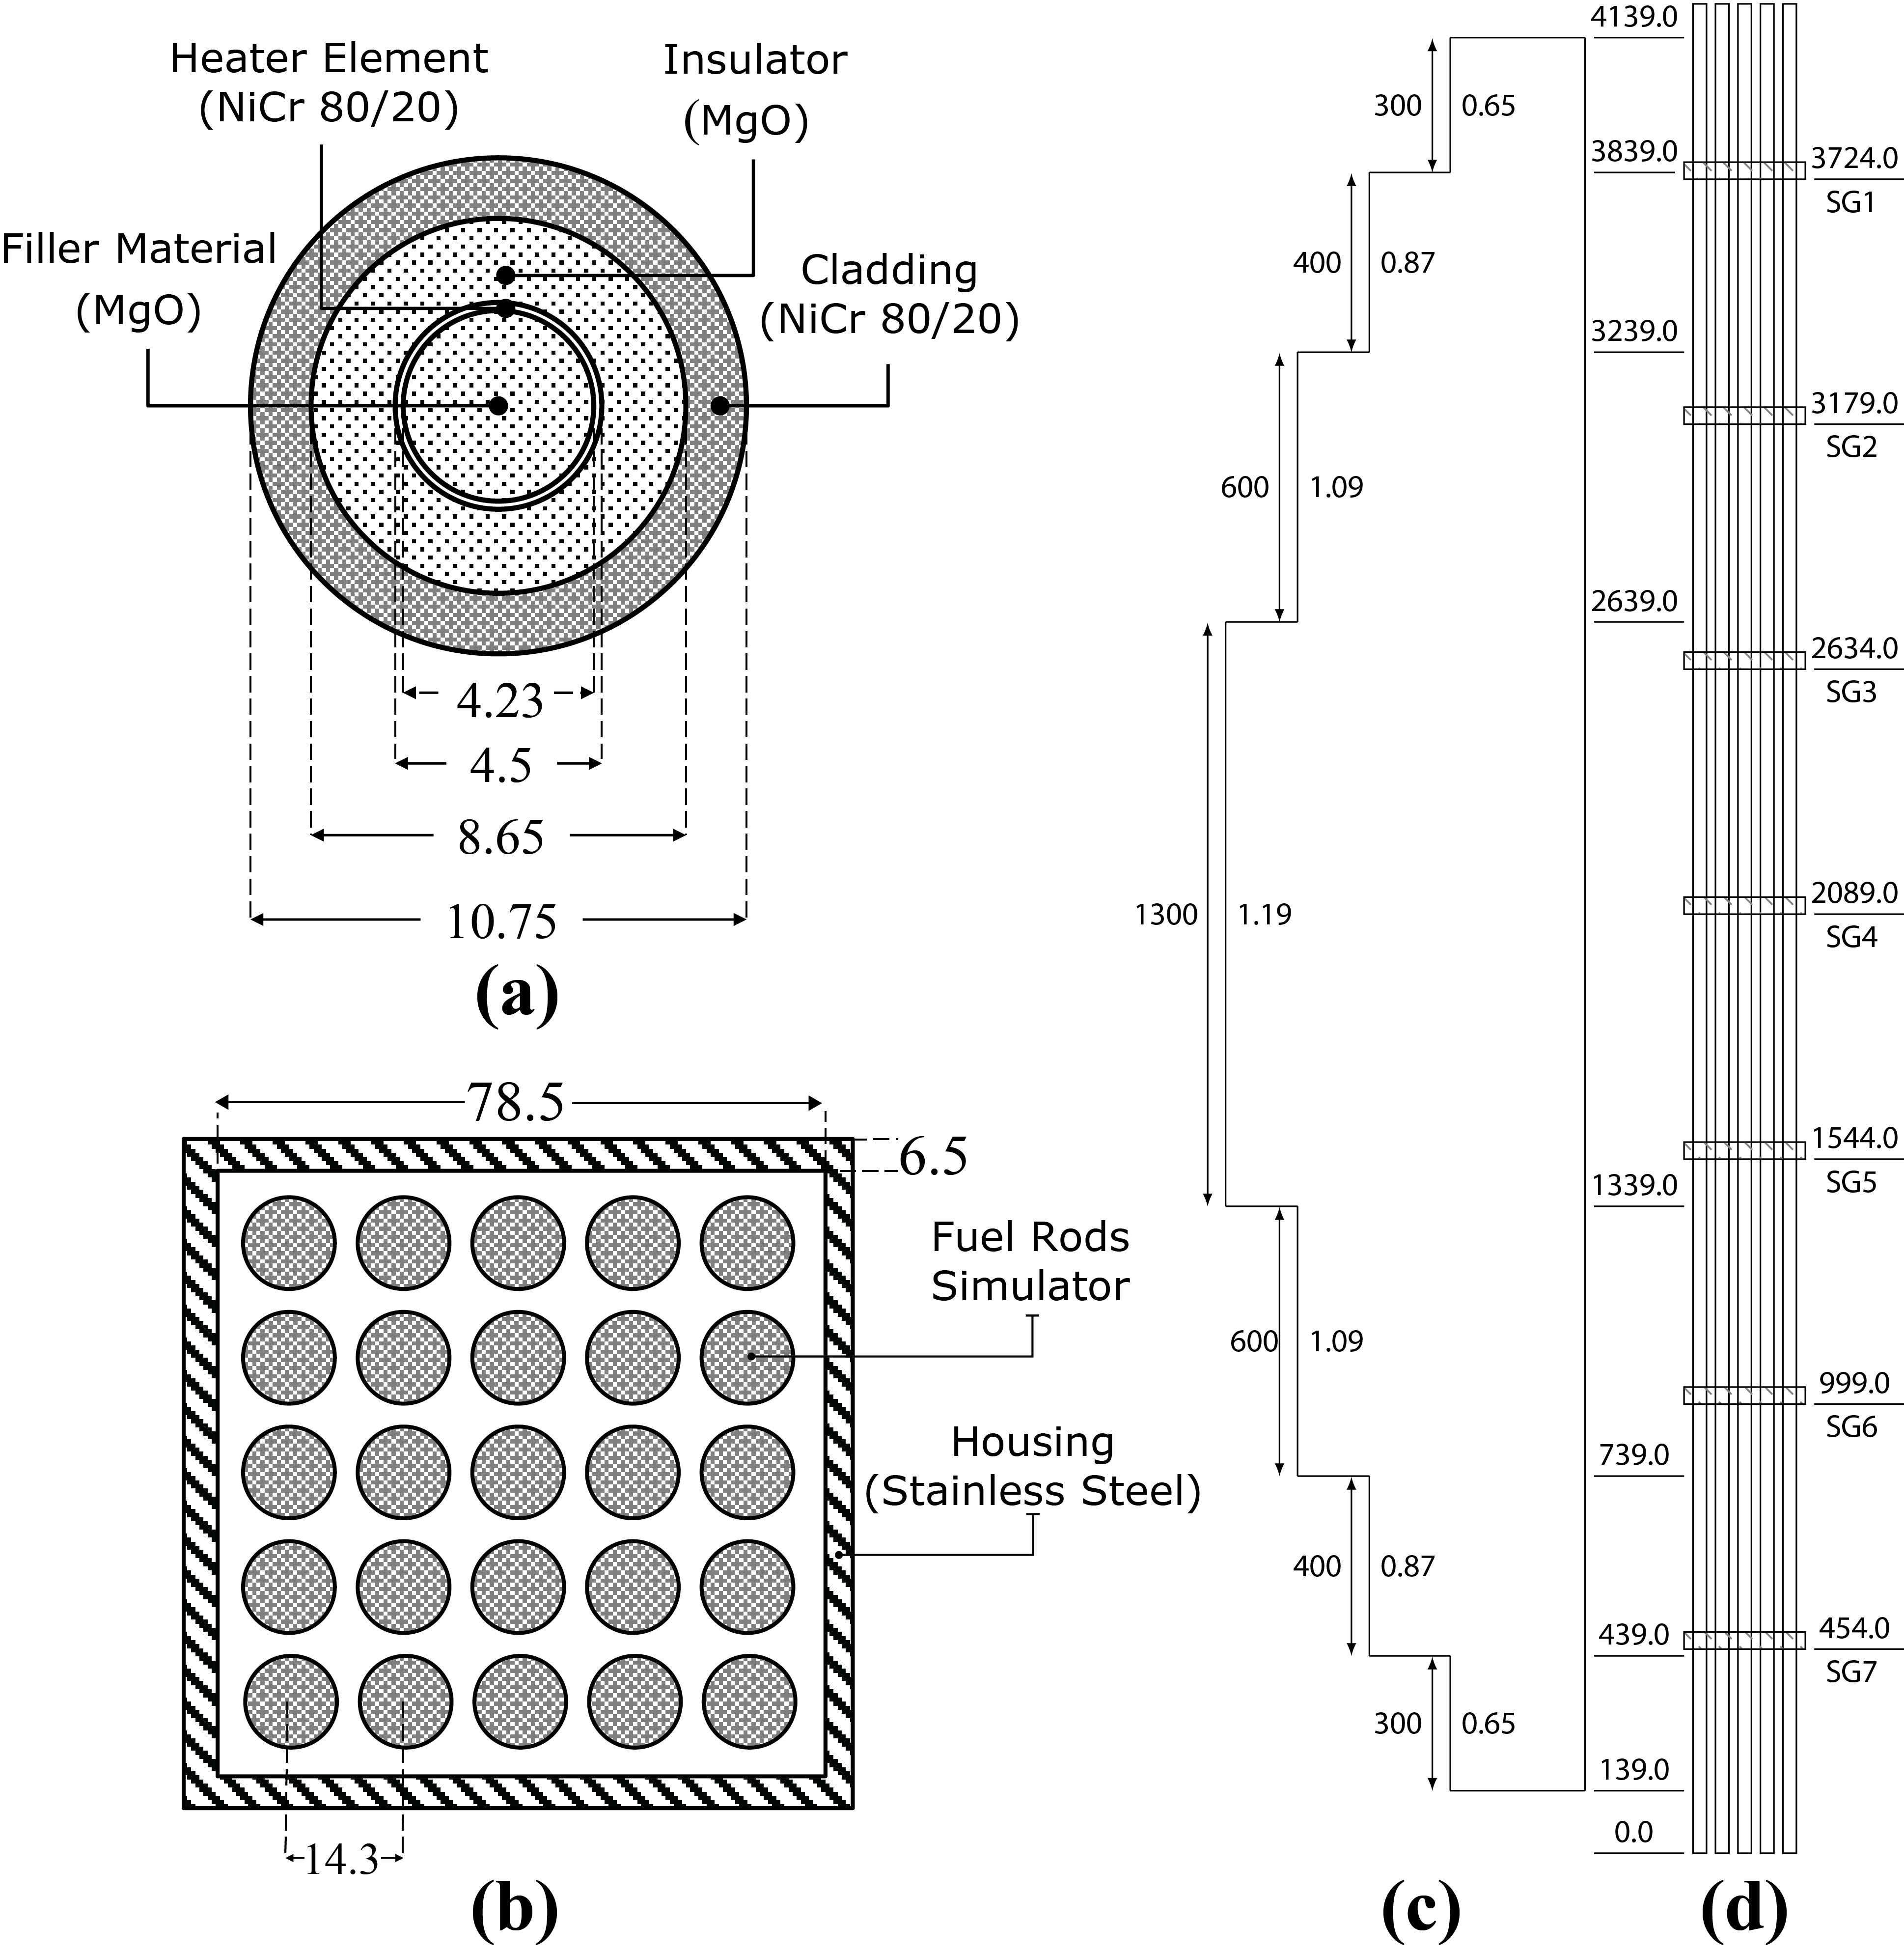
\includegraphics[width=1.0\textwidth]{../figures/febaTestSection/febaTestSection.png}
	\caption[FEBA experimental facility]{(a) The cross section of the fuel rod simulators used in \gls[hyper=false]{feba} separate-effect test facility. (b) the cross section of the test section including the rectangular housing. (c)  The approximate cosine power profile, numbers written inside the bix are the relative power $P/P_{avg}$. (d) The location of spacer grids in the test section. All dimensions are in units of milimeters $[mm]$}\label{fig:feba_setf}
\end{figure}

% How the experiment was conducted
During the initialization phase of the experiment,
the test section was heated up at low nominal power ($200 \ [kW]$) to achieve a specified initial heater rod temperature, with no liquid present in the test section.
The transient phase of the experiment was initiated by ramping up the power according to $120$\% (ANS\footnote{American National Standard}) decay heat power curve while simultaneously injecting subcooled liquid from the bottom of the test section.
Several temperature measurements at the outer surface of the heater rods, hereinafter referred to as the clad temperature, were taken at different axial locations during the course of each transient test.

% FEBA Test Series
Eight different test series were performed in the FEBA facility. 
The first two test series (I and II) used two different numbers of spacer grids, seven and six, respectively.
The middle spacer grid was removed in test series II to investigate the effect of spacer grids in a reflood transient.
The other test series used different flow area blockage sizes at midheight of the test section to investigate the effect of rod ballooning of different sizes.
In each test series, combinations of two different inlet liquid velocities and three different system backpressure were imposed.

% FEBA Test Series I
The present thesis analyzed only the experimental data sets from the test series I.
This particular test run was used as the base experimental setup with all seven spacer grids mounted and no flow area blockage.
Different experimental runs corresponding to different experimental conditions of test series I are given in Table~\ref{tab:feba_exp}.

\begin{table}[h]
	\myfloatalign
	\caption[FEBA Test Series I Experimental Conditions]{FEBA Test Series I Experimental Conditions}
	\label{tab:feba_exp}
	\begin{tabularx}{\textwidth}{ccc} \toprule
		\tableheadline{FEBA Test No.} & \tableheadline{System Pressure} & \tableheadline{Flooding Rate} \\ 
		                              & $[bar]$                         & $[cm \cdot s^{-1}]$ \\ \midrule
		216 & $4.12$  & $3.81$ \\
		214 & $4.11$  & $5.77$ \\
		223 & $2.21$  & $3.82$ \\
		218 & $2.08$  & $5.81$ \\
		220 & $6.18$  & $3.85$ \\
		222 & $6.18$  & $5.78$ \\
		\bottomrule
	\end{tabularx}
\end{table}

% Source of FEBA Information
The facility specification and the test data are compiled in a series of reports that are available at the KIT library website.
The specifications and the data provide a valuable source of information for \gls[hyper=false]{trace} code assessment since the \gls[hyper=false]{feba} experiment is not part of the original validation matrix of the code. 
More details can be found in \cite{Ihle1984}.
\section{FEBA Model in TRACE}\label{sec:reflood_feba_trace}

The \textsc{FEBA} facility was modeled using the TH system code \textsc{TRACE}.
The model consists of a one-dimensional \textsc{VESSEL} component (to model the bundle test section),
a \textsc{PIPE} component (upper plenum of the test section), 
a \textsc{FILL} component (inlet flow and inlet temperature boundary conditions),
a \textsc{BREAK} component (outlet pressure boundary condition),
two \textsc{HTSTR} components (heater rods simulator and non-powered test section housing),
and a \textsc{POWER} components (imposed electrical boundary condition).

The \textsc{VESSEL} component was nodalized into $28$ hydraulic nodes of varying sizes between $60$ and $315$ $[mm]$.
Both \textsc{HTSTR} components were also nodalized into the sample number of coarse axial conduction nodes.
However, since a large axial temperature gradient is expected in a reflood transient,
the fine-mesh reflood flag in \textsc{TRACE} was enabled.
As a result, each of the course conduction nodes is divided uniformly by $5$,
yielding a total of $142$ axial conduction nodes.
The main geometrical parameters and experimental conditions used to develop the \textsc{FEBA} input model
are summarized in Table~\ref{tab:feba_trace}.

\begin{table}[ht]
    \myfloatalign
    \caption[]{Geometrical parameters and experimental conditions for the \gls{feba} model in \gls{trace}}  \label{tab:feba_trace}
    \begin{tabularx}{\textwidth}{Xcc} \toprule
        \tableheadline{Parameter}		& \tableheadline{Unit} & \tableheadline{Value} \\ \midrule
        Test section total length 		& $[m]$		& $4.114$ \\
        Total heated length 			& $[m]$		& $3.9$ \\
        Flow area						& $[m^2]$	& $3.901 \times 10^{-3}$\\
        Hydraulic diameter				& $[mm]$	& $13.45$\\
        Rectangular housing width   	& $[mm]$	& $78.55$\\
        Rectangular housing thickness	& $[mm]$	& $6.5$\\
        Number of rods					& $[-]$		& $25$\\
        Rod outer diameter				& $[mm]$	& $10.75$\\
        Pitch-to-Diameter ratio			& $[-]$		& $1.33$\\
        Number of spacer grids			& $[-]$		& $7$\\
        Spacer grid flow obstruction	& $[\%]$	& $20$\\
        Spacer grid axial locations		& $[m]$		& $7$\\
        \midrule
        Number of hydraulic nodes		& $[-]$		& $28$ (varying length)\\
        \multirow{2}{*}{Number of axial nodes}   		& \multirow{2}{*}{$[-]$}		& $28$ (coarse)\\
                                		&   		& $142$ (fine)\\
        \midrule
        Inlet liquid temperature        & $[K]$		&  $312$ \\
        Inlet flow velocity				& $[cm\cdot s^{-1}]$ & see Table~\ref{tab:feba_exp} \\
        System backpressure             & $[bar]$   & see Table~\ref{tab:feba_exp} \\
        \bottomrule
    \end{tabularx}
\end{table}

\subsection{Base Case Simulation Results}

\subsection{Prior Uncertainty Propagation}

%******************************************************************************************
\section{Initial Selection of Input Parameters}\label{sec:reflood_initial_inputs_selection}
%******************************************************************************************

% Introductory paragraph
This section presents the selection process of the initial set of uncertain input parameters of the \gls[hyper=false]{feba} simulation in \gls[hyper=false]{trace}.
Afterward, the assignment of the initial (prior) uncertainties of these parameters are presented. 
This part is closely related to PSI participation in the \gls[hyper=false]{premium} benchmark thus several reference are made to activities related to that benchmark \cite{Zerkak2016}.

%---------------------------------------------------------------------------------
\subsection{Selection of Input Parameters}\label{sub:reflood_parameters_selection}
%---------------------------------------------------------------------------------

% Introductory paragraph
The selection process for the uncertain input parameters to consider differs depending on the type of parameter.
Each of the selected parameters can broadly fall into one of the two following categories:
\begin{itemize}
	\item Input parameters that are not specific to the \gls[hyper=false]{trace} code (e.g., initial and boundary conditions, material thermo-physical properties).
		This category of parameters is often referred to as the \emph{controllable inputs} of the simulation.
	\item Input parameters that are specific to \gls[hyper=false]{trace} code (e.g., implementation of the two-phase momentum and heat transfer package for reflood condition).
		This category is often referred to as the \emph{model parameters} of the simulation.
\end{itemize}

% Selection on the first category
The selection of parameters belonging to the controllable inputs category simply corresponds to the parameters recommended by the benchmark organizers and employed by most participants \cite{Kovtonyuk2015}.
The $13$ selected parameters of this category are listed in Table~\ref{tab:trace_model_parameter_1}.

% Selection on the second category
On the other hand, the selection of the model parameters specific to the \gls[hyper=false]{trace} code is challenging due to the fact that \gls[hyper=false]{trace} is a relatively recent code (in comparison with codes like RELAP5, ATHLET, or CATHARE).
In essence, the code has been developed from different variants of the TRAC codes for different reactor types (TRAC-BF1, TRAC-P) to result in a single consolidated code applicable to both \gls[hyper=false]{pwr} and \gls[hyper=false]{bwr}.
Contributing to that difficulty is the fact that \gls[hyper=false]{trace} is currently undergoing significant developments and improvements, including modifications to the two-phase closure models for momentum and heat transfers.
Consequently, the task of selecting the model parameters and later their prior uncertainties is more difficult than for a more established codes.

% Criteria for choosing the parameters
To overcome this issue, the following principles have been followed to select the model parameters:
\begin{enumerate}
	\item The selection has been focused on the physical models in the post-\glsentryshort{chf} package of the \gls[hyper=false]{trace} code (including the reflood models).
		Specifically, these are models for the \gls[hyper=false]{iafb} and \gls[hyper=false]{dffb} flow regimes \cite{USNRC2012}.
	\item Spacer grid model are also included as they are known to have a significant impact on reflooding \cite{Miller2013}.
	\item Parameters related to the minimum film boiling temperature and transition boiling should be selected, since they have (by model construction) an impact on the time of quenching.
\end{enumerate}

Additionally, as a common principle, the selected models (and parameters) are to be perturbed by means of perturbation factors (detail below) at the highest-possible level of the structure of these model.
This allows, to some extent, to use reference uncertainty information obtained from codes other than \gls[hyper=false]{trace}.

% Resulting List of Model Parameters 1
In accordance with the first selection principle above, a set of $10$ high-level parameters has been selected ($5$ for each flow regime).
Specifically, for each flow regime: the wall-fluid \gls[hyper=false]{htc}, the liquid-interface \gls[hyper=false]{htc}, the vapor-interface \gls[hyper=false]{htc}, the wall-fluid drag coefficient, and the interfacial drag coefficient.

% Resulting List of Model Parameters 2
Following the second principle, two additional parameters have been selected:
the spacer grid pressure loss coefficient model from Yao, Loftus, and Hochreiter as well as the grid convective \gls[hyper=false]{ht} enhancement model from Yao, Hochreiter, and Leech (see \cite{USNRC2012} pp. $425$--$429$ and \cite{Yao1982}).
These perturbations on the parameters are applied to all seven spacer grids at once.

% Resulting List of Model Parameters 3
Lastly, from the third principle, the quench temperature parameter in \gls[hyper=false]{trace} and wall-fluid \gls[hyper=false]{htc} for transition boiling (see \cite{USNRC2012} pp. $293$--$299$) have been added to the list of uncertain input parameters.

In the end, fourteen parameters are and are summarized in Table~\ref{tab:trace_model_parameter_2}.
The total number of initial uncertain input parameters considered is thus $27$.

% Table Input Parameters
\begin{sidewaystable}

\caption{Selected \gls[hyper=false]{trace} input parameters (controllable inputs), their perturbation factors and their range of variations.}
\label{tab:trace_model_parameter_1}
\centering
\newcolumntype{Y}{>{\RaggedRight\arraybackslash}X}
%\begin{tabularx}{\textwidth}{@{}c|>{$}c<{$}|>{$}c<{$}|Y|Y|Y|Y|Y@{}}
\begin{tabularx}{0.985\textwidth}{@{}cccc>{$}c<{$}>{$}c<{$}c@{}}
\toprule
No.	& Parameter 				& Description 										& Distribution & \text{Range of}  & \text{Nominal} & Mode of \\
		& ID        				&                             		&              & \text{Variation} & \text{Value}   & Perturbation \\
\midrule
1  	& \texttt{breakP} 	& Outlet pressure 								& Uniform 	& [0.90, 1.10]   	& 1.0 			& Multiplicative \\ 
2  	& \texttt{fillT} 		& Inlet water temperature 				& Uniform 	& [-5.00, +5.00] 	& 0.0\,[K] 	& Additive \\ 
3  	& \texttt{fillV}		& Inlet water velocity          	& Uniform 	& [0.90, 1.10]   	& 1.0 			& Multiplicative \\ 
4  	& \texttt{pwr} 			& Heater rod power             	 	& Uniform 	& [0.90, 1.05]   	& 1.0 			& Multiplicative \\ 
\midrule
5  	& \texttt{nicK} 		& Conductivity (Nichrome) 				& Uniform 	& [0.95, 1.05] 		& 1.0 			& Multiplicative \\ 
6  	& \texttt{nicCP} 		& Specific heat (Nichrome)				& Uniform 	& [0.95, 1.05] 		& 1.0 			& Multiplicative \\ 
7  	& \texttt{nicEM} 		& Emissivity (Nichrome) 					& Uniform 	& [0.90, 1.00] 		& 0.95			& Substitutive \\ 
8  	& \texttt{mgoK} 		& Conductivity (MgO)							& Uniform 	& [0.80, 1.20] 		& 1.0 			& Multiplicative \\
9  	& \texttt{mgoCP}		& Specific heat (MgO) 						& Uniform 	& [0.80, 1.20] 		& 1.0 			& Multiplicative \\ 
10 	& \texttt{vesEps}		& Wall roughness 									& Uniform 	& [6.10\times 10^{-7}, 2.44\times 10^{-6}] & 1.5 \times 10^{-6} \, [m] & Substitutive \\ 
11 	& \texttt{ssK} 			& Conductivity (stainless steel)	& Uniform 	& [0.95, 1.05] 		& 1.0 			& Multiplicative \\ 
12 	& \texttt{ssCP} 		& Specific heat (stainless steel)	& Uniform		& [0.95, 1.05] 		& 1.0 			& Multiplicative \\ 
13 	& \texttt{ssEM} 		& Emissivity (stainless steel)		& Uniform 	& [0.56, 0.94] 		& 0.84 			& Substitutive \\ 
\bottomrule
\end{tabularx}
\end{sidewaystable}


\begin{sidewaystable}

\caption{Selected \gls[hyper=false]{trace} input parameters (model parameters), their perturbation factors and their range of variations}
\label{tab:trace_model_parameter_2}

\centering
\newcolumntype{Y}{>{\RaggedRight\arraybackslash}X}
%\begin{tabularx}{\textwidth}{@{}c|>{$}c<{$}|>{$}c<{$}|Y|Y|Y|Y|Y@{}}
\begin{tabularx}{0.90\textwidth}{@{}cccc>{$}c<{$}>{$}c<{$}c@{}}
\toprule
No. & Parameter 							& Description & Distribution & \text{Range of}  & \text{Nominal} & Mode of \\
    & ID        							&             &              & \text{Variation} & \text{Value}   & Perturbation \\
\midrule
14 	& \texttt{gridK} 					& Spacer grid $\Delta p$ coefficient															& Uniform 				& [0.25, 1.75] 		& 1.0 				& Multiplicative \\ 
15  & \texttt{gridHT} 				& Spacer grid \gls[hyper=false]{htc} enhancement									& Log-Uniform 		& [0.50, 2.00] 		& 1.0				 	& Multiplicative \\ 
16  & \texttt{iafbWHT}  			& Wall \gls[hyper=false]{htc} (\glsentryshort{iafb})							& Log-Uniform 		& [0.50, 2.00]   	& 1.0 				& Multiplicative \\ 
17  & \texttt{dffbWHT}  			& Wall \gls[hyper=false]{htc} (\glsentryshort{dffb})  						& Log-Uniform 		& [0.50, 2.00] 	  & 0.0 				& Multiplicative \\ 
18  & \texttt{iafbLIHT}				& Liquid-interface \gls[hyper=false]{htc} (\glsentryshort{iafb})  & Log-Uniform 		& [0.25, 4.00]   	& 1.0 				& Multiplicative \\ 
19  & \texttt{iafbVIHT} 			& Vapor-interface \gls[hyper=false]{htc}  (\glsentryshort{iafb})  & Log-Uniform 		& [0.25, 4.00]   	& 1.0 				& Multiplicative \\ 
20  & \texttt{dffbLIHT} 			& Liquid-interface \gls[hyper=false]{htc} (\glsentryshort{dffb}) 	& Log-Uniform 		& [0.25, 4.00] 	 	& 1.0 				& Multiplicative \\ 
21  & \texttt{dffbVIHT} 			& Vapor-interface \gls[hyper=false]{htc} (\glsentryshort{dffb})	 	& Log-Uniform 		& [0.25, 4.00] 	 	& 1.0 				& Multiplicative \\ 
22  & \texttt{iafbIntD} 			& Interfacial drag (\glsentryshort{iafb}) 												& Log-Uniform 		& [0.25, 4.00] 	 	& 1.0 				& Multiplicative \\ 
23  & \texttt{dffbIntDr} 			& Interfacial drag (\glsentryshort{dffb})													& Log-Uniform 		& [0.25, 4.00]		& 1.0 				& Multiplicative \\
24  & \texttt{iafbWallDr} 		& Wall drag (\glsentryshort{iafb}) 																& Log-Uniform 		& [0.50, 2.00] 		& 1.0 				& Multiplicative \\ 
25	& \texttt{dffbWallDr} 		& Wall drag (\glsentryshort{dffb})			  												& Log-Uniform 		& [0.50, 2.00] 		& 1.0 				& Multiplicative \\ 
26 	& \texttt{transHTCWallSV}	& Wall \gls[hyper=false]{htc} (Transition boiling)								& Log-uniform			& [0.25, 4.00] 		& 1.0 				& Multiplicative \\ 
27 	& \texttt{tQuench} 				& Quenching temperature $[K]$																			& Uniform 				& [-50.0, +50.0] 	& 0.0 \, [K]	& Additive \\ 
\bottomrule

\end{tabularx}
\end{sidewaystable}

%----------------------------------------------------------------------------------
\subsection{Perturbation Factors}\label{sub:reflood_parameters_perturbation_factor}
%----------------------------------------------------------------------------------

% Opening paragraph
The nominal values of the selected input parameters of the \gls[hyper=false]{trace} \gls[hyper=false]{feba} model are varied by means perturbation factors.
These perturbation factors are modeled as random variables following a predefined \gls[hyper=false]{pdf} detailed in the next section, from which a set of samples of input parameters values can be generated.

% Mode of perturbations
For a given sampled perturbation factor, one of three modes of perturbation is possible: \emph{additive}, \emph{multiplicative,} and \emph{substitutive}.
In the additive mode, the sampled perturbation factor is added to the nominal parameter value of the \gls[hyper=false]{trace} model.
In the multiplicative mode, the sampled perturbation factor is multiplied by the nominal parameter value.
Finally, in the substitutive mode, the sampled perturbation factor directly substitutes for the nominal parameter value.
The mode of perturbation for each selected input parameter are listed in last column of Table~\ref{tab:trace_model_parameter_1} and Table~\ref{tab:trace_model_parameter_2}.

% trace-simexp
A tool is developed in the Python programming language to assist in automatically pre-processing, executing, and post-processing numerous \gls[hyper=false]{trace} simulations of the \gls[hyper=false]{feba} model based on a set of sampled input parameters values.
The tool, \texttt{trace-simexp}, is detailed in Appendix~\ref{app:trace_simexp}.

%-----------------------------------------------------------------------------------
\subsection{Prior Uncertainty Quantification}\label{sub:reflood_parameters_prior_uq}
%-----------------------------------------------------------------------------------

% Opening Paragraph
The uncertainties associated with the controllable inputs were taken directly from the recommended value of the \gls[hyper=false]{premium} benchmark and the list can be found in Table~\ref{tab:trace_model_parameter_1}.
As for the model parameters, a first determination of the uncertainty ranges has been made following an internal selection process primarily based on the use of information in available literature on uncertainties in physical models for \gls[hyper=false]{lbloca}.

% Main Source of Information
The main sources of information consisted of Ref.\cite{Wickett1991} and Ref.~\cite{Glaeser2008a} which included uncertainty information for the closure models of system codes TRAC-PF1/MOD1 and ATHLET-Mod2.1 (Cycle B), respectively. 
Furthermore, prior experience and knowledge of the closure model uncertainties of the CATHARE2 code (\texttt{V1.3L\_1}, Rev.5) has been used \cite{Zerkak2016,IPSN2001}.
Ref.~\cite{IPSN2001} accounts an analysis by IPSN\footnote{Institut de protection et de s\^{u}ret\'e nucl\'eaire (IPSN)} of the uncertainty quantification method ``M\'ethode D\'eterministe R\'ealiste'' for the \gls[hyper=false]{pwr} \gls[hyper=false]{lbloca} which was proposed by EDF\footnote{Electricit\'e de France} and was evaluated in $2000$.
The high-level implementation of the perturbation factors for the uncertainty analysis in the post-\gls[hyper=false]{chf} closure models, allowed information from different codes to be extracted for the initial estimate.
This approach was deemed adequate in the limited context of the determination of the prior \glspl[hyper=false]{pdf}.

% Uniform and Log-Uniform
To simplify the quantification of the prior uncertainties further, and for the multiplication factor, the \glspl[hyper=false]{pdf} were assumed to follow a symmetric bounded uniform and log-uniform distributions with the nominal parameter value as the median value.
For the log-uniform distribution the form $[2^{-n}, 2^{n}]$ was assumed, where $n$ an integer.
All \glspl[hyper=false]{pdf} of model parameters that were a priori deemed to be important were of log-uniform distribution.

The ranges of the parameters (i.e., their minimum and maximum), were determined so as to cover the information available for a similarly (or judged to be related) parameter in Refs.~\cite{Wickett1991,Glaeser2008a}.
Though this at times resulted in the selection of a large bound, they were deemed acceptable following a verification study against the nominal predictions.
The verification heavily relied on engineering judgment via visual inspection of the width of the predictions uncertainty bands to decide if the width due to the assumed parameter uncertainties were indeed reasonable\footnote{The loosely defined notion of ``reasonable'' in this case is similar to the notion of ``'behavioral vs. non-behavioral'' prediction in hydrology modeling \cite{Beven2009}.}.
At that point, the approach was admitedly imprecise, but it was intentional in the general context of determining the prior range, especially to avoid mistakenly underestimating the uncertainties associated with influential model parameters. 

%
Table~\ref{tab:trace_model_parameter_2} lists the results of the prior uncertainty quantification of the selected model parameters.

%***************************************************************************
\section{Propagation of the Prior Uncertainties}\label{sec:reflood_prior_uq}
%***************************************************************************

Hence, the \emph{prior uncertainty propagation} step constitutes of generating samples for each model parameter from its prior \gls[hyper=false]{pdf}, 
carrying out a set of \gls[hyper=false]{trace} simulations of the \gls[hyper=false]{feba} model using the sampled parameters, 
and analyzing the results to quantify the uncertainty of the model prediction.

% Make observation about variation in time and amplitude
% The data seems to be within TRACE parametrization, regardless whether they are consistent or not.

% FEBA Test No. 216 Prior Uncertainty Propagation, TC
\begin{sidewaysfigure}
	\centering
	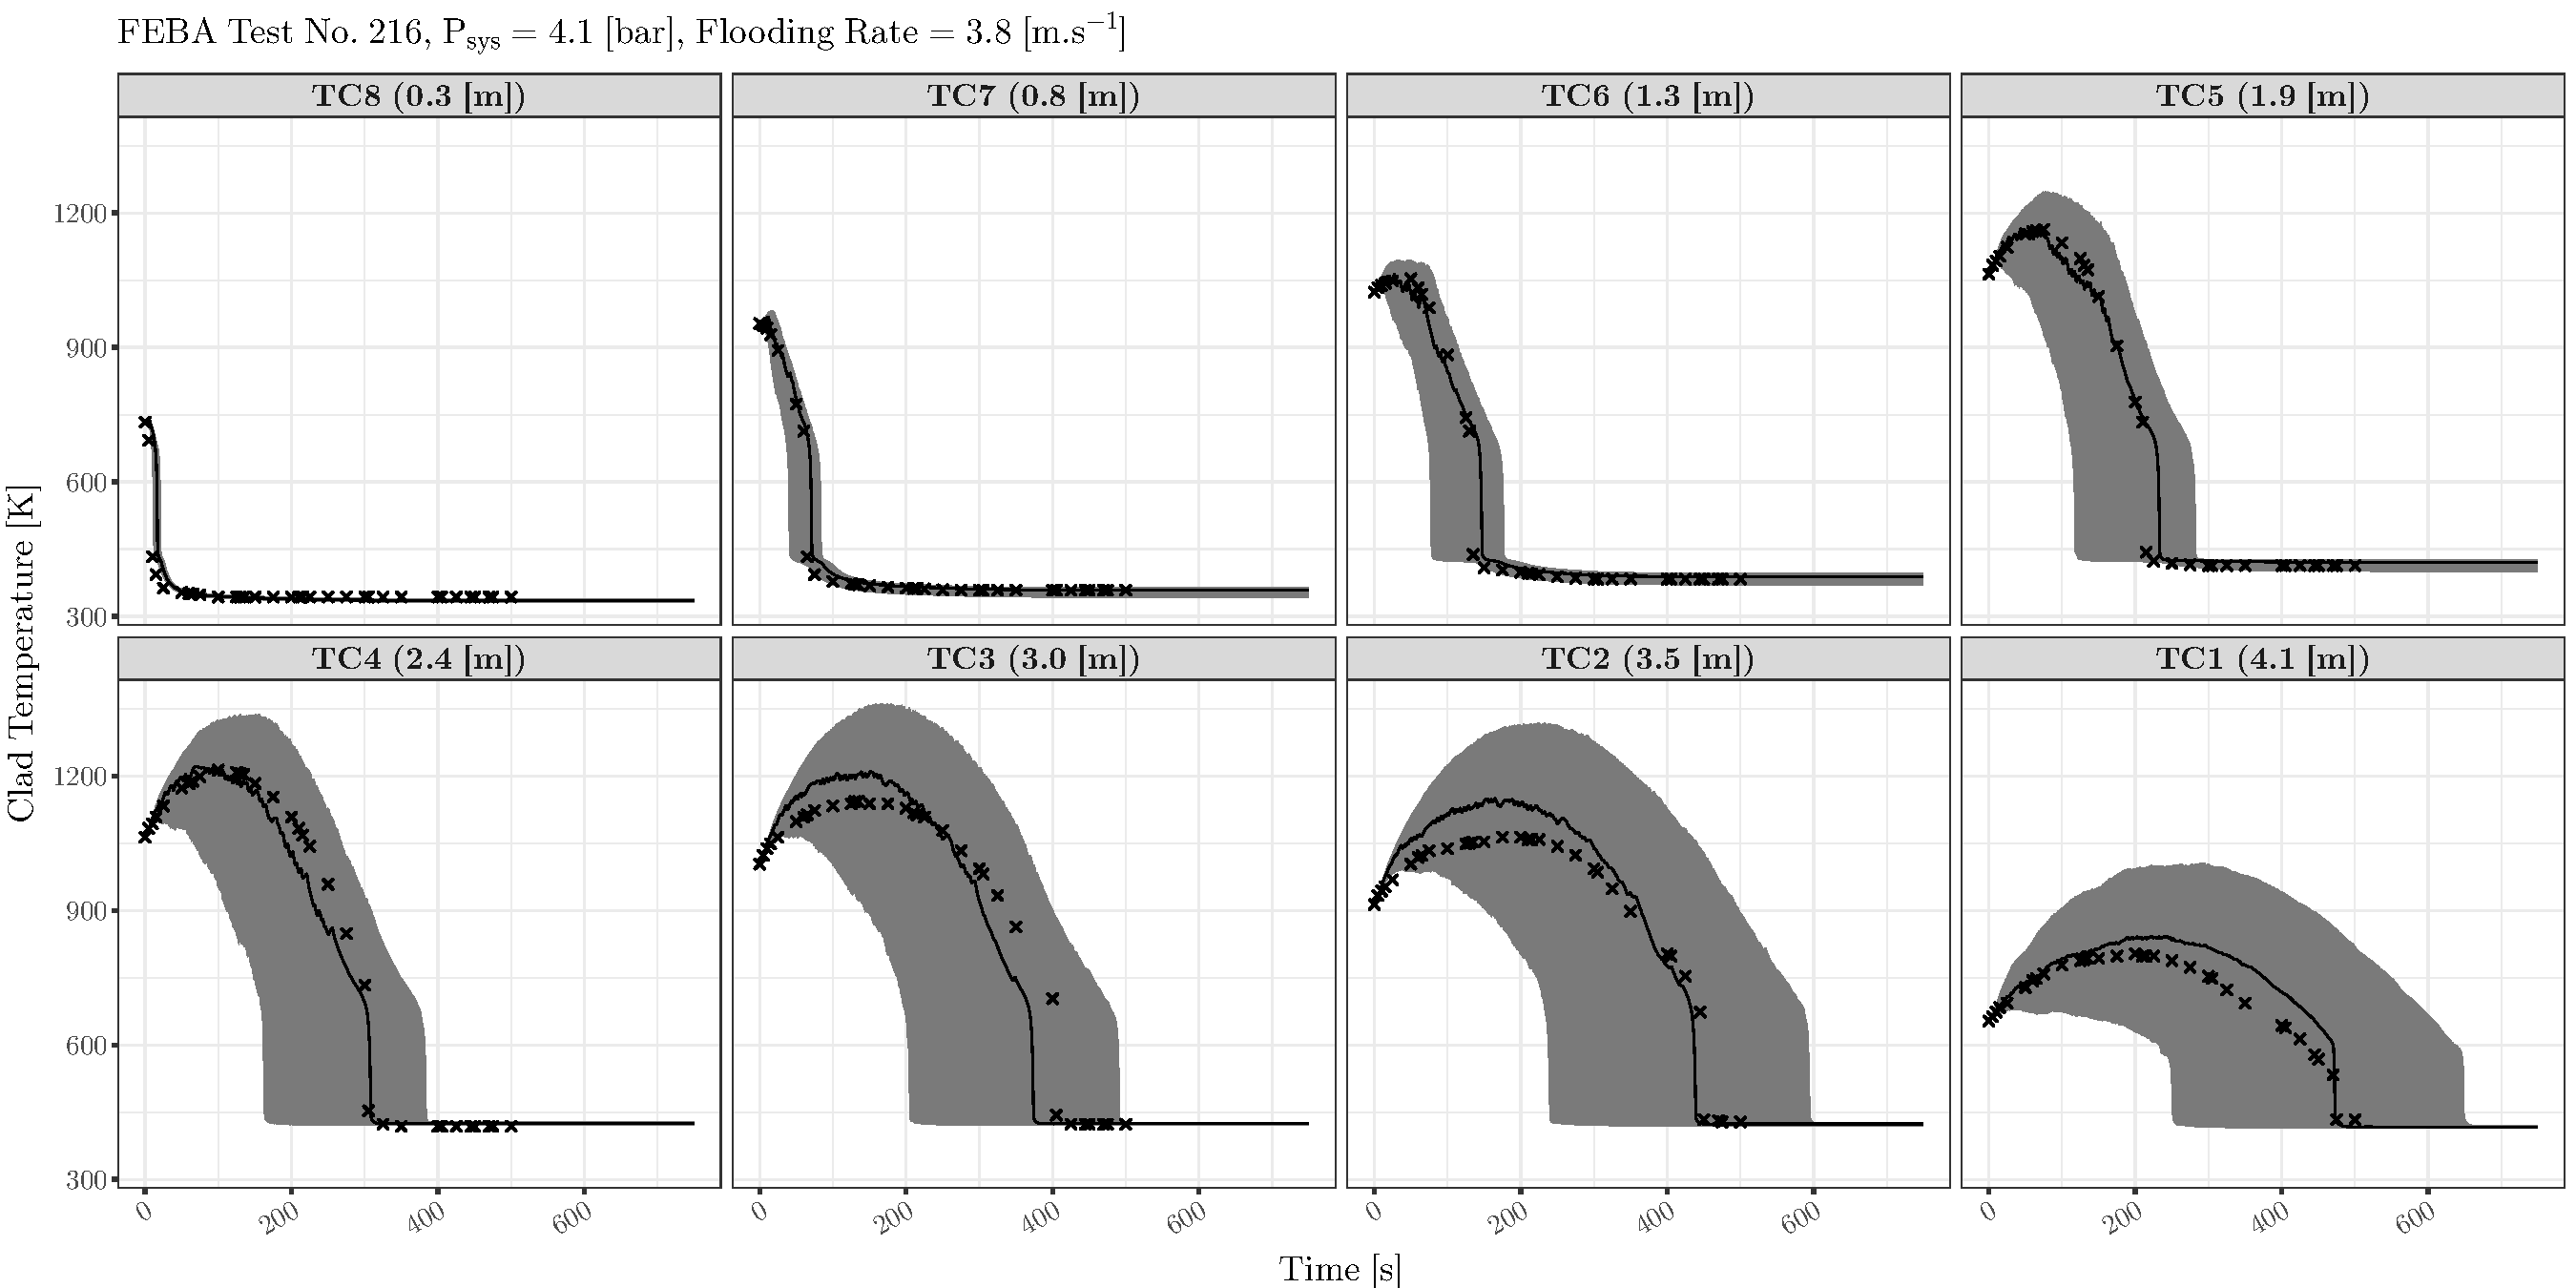
\includegraphics[width=0.90\textwidth]{../figures/chapter2/figures/plotTraceUQPriorTC216}
		\captionof{figure}[Propagation of the $27$ input parameters prior uncertainties on FEBA test No. $216$ for the cladding temperature output ($TC$).]{Propagation of the $27$ input parameters prior uncertainties on FEBA test No. $216$ for the cladding temperature output ($TC$). The uncertainty bound corresponds to the symmetric ($95\%$) probability; solid lines and crosses indicate the simulation with the nominal parameters values and the experimental data, respectively.}
	\label{fig:ch2_plot_trace_uq_prior_tc_216}
\end{sidewaysfigure}


% FEBA Test No. 216 Prior Uncertainty Propagation, DP
\begin{figure}[bth]
    \centering
    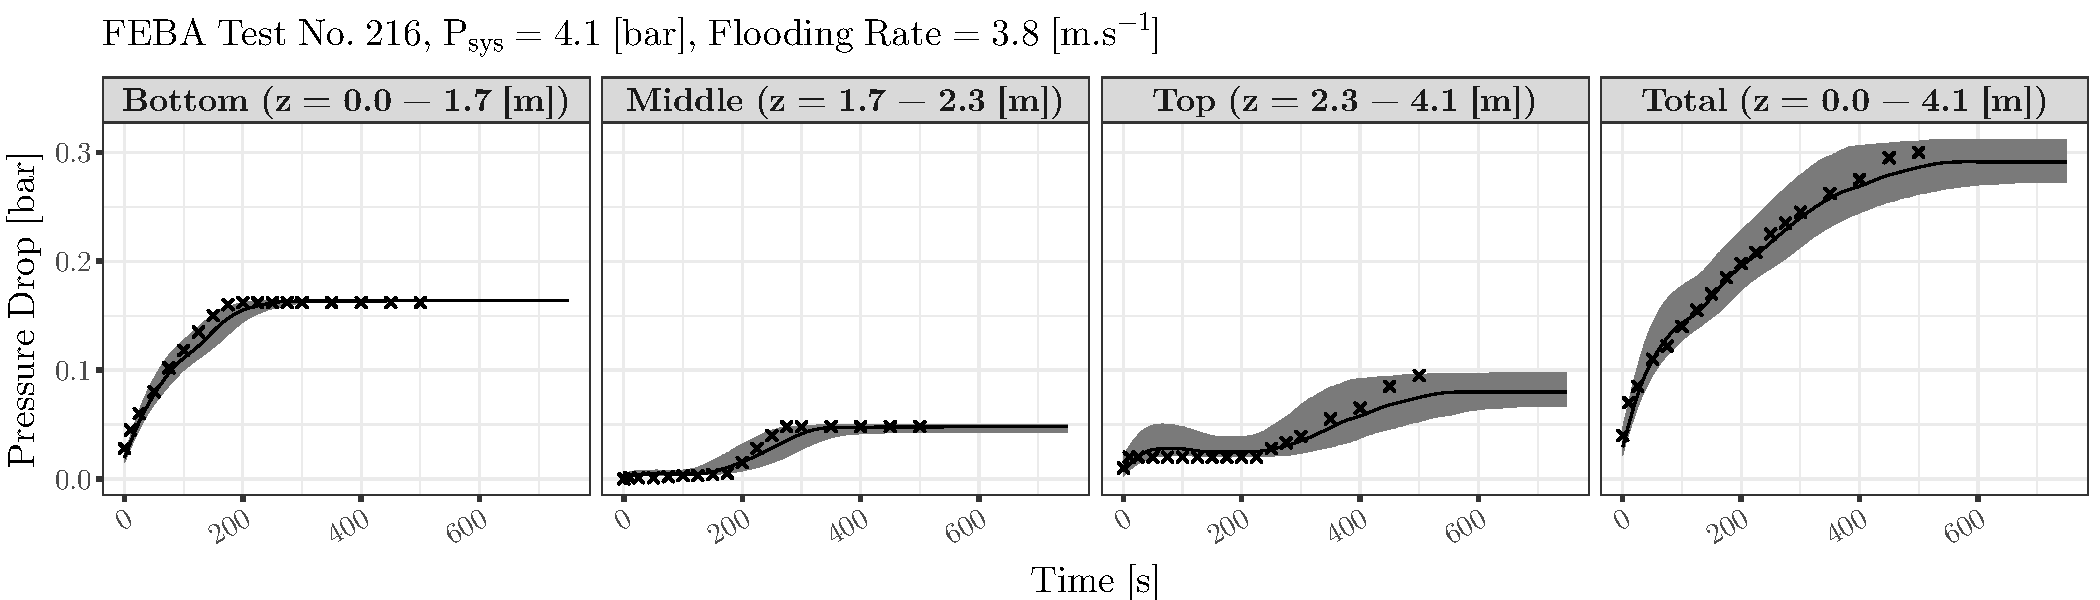
\includegraphics[width=1.0\textwidth]{../figures/chapter2/figures/plotTraceUQPriorDP216}
    \caption[Propagation of the $27$ input parameters prior uncertainties on FEBA test No. $216$ for the pressure drop output ($DP$).]{Propagation of the $27$ input parameters prior uncertainties on FEBA test No. $216$ for the pressure drop output ($DP$). The uncertainty bound corresponds to the symmetric ($95\%$) probability; solid lines and crosses indicate the simulation with the nominal parameters values and the experimental data, respectively.}
    \label{fig:ch2_plot_trace_uq_prior_dp_216}
\end{figure}

\begin{figure}[!bth]
    \centering
    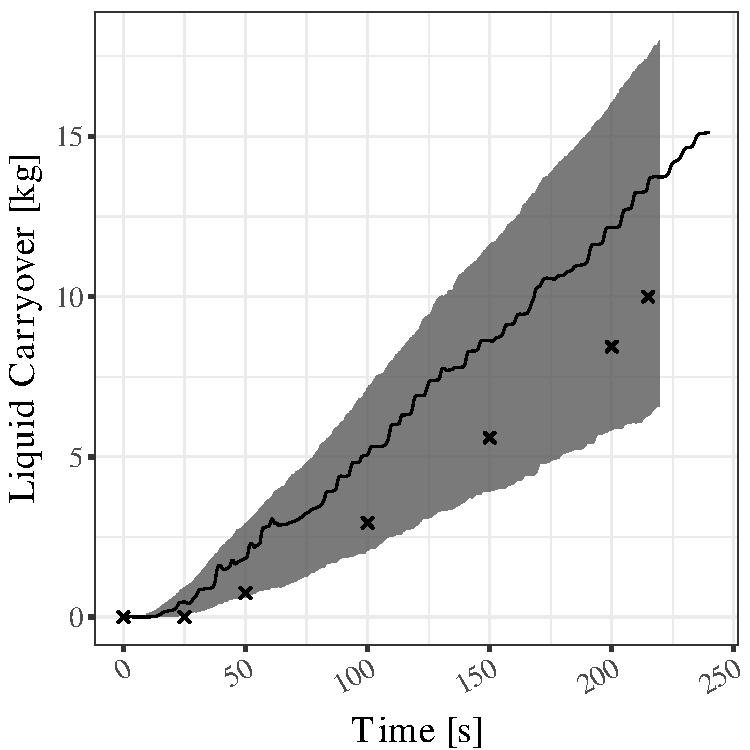
\includegraphics[width=0.5\textwidth]{../figures/chapter2/figures/plotTraceUQPriorCO216}
    \caption[Propagation of the $27$ input parameters prior uncertainties on FEBA test No. $216$ for the liquid carryover output ($CO$).]{Propagation of the $27$ input parameters prior uncertainties on FEBA test No. $216$ for the pressure drop output ($CO$). The uncertainty bound corresponds to the symmetric ($95\%$) probability; solid lines and crosses indicate the simulation with the nominal parameters values and the experimental data, respectively.}
    \label{fig:ch2_plot_trace_uq_prior_co_216}
\end{figure}
\section{Chapter Summary}\label{sec:sa_chapter_summary}
Illo principalmente su nos. Non message \emph{occidental} angloromanic
da. Debitas effortio simplificate sia se, auxiliar summarios da que,
se avantiate publicationes via. Pan in terra summarios, capital
interlingua se que. Al via multo esser specimen, campo responder que
da. Le usate medical addresses pro, europa origine sanctificate nos
se.
%************************************************************
